\documentclass[11pt]{report}
\usepackage[utf8]{inputenc}
\usepackage[margin=2.0cm]{geometry}
\usepackage{fancyhdr}
\usepackage{xcolor}
\usepackage{minted}
\usepackage{graphicx}
\usepackage[parfill]{parskip}

\title{Digital Engineering\\Lab 3}
\author{Y3890959\\Y3878784}
\date{7th February 2023}

\pagestyle{fancy}
\fancyhead{}
\setlength{\headheight}{14pt}
\fancyhead[L]{Lab 3}
\fancyhead[R]{Y3890959, Y3878784}
\fancyfoot{}
\fancyfoot[L]{Digital Engineering}
\fancyfoot[R]{\thepage}

\makeatletter
\let\ps@plain\ps@fancy 
\makeatother

\setminted {
    fontsize=\footnotesize,
    frame=single,
}

\begin{document}

\maketitle

\chapter*{Task A: Pipelining}

\section*{2.1.1 Behaviour Simulation}
\subsection*{Waveform 1: Global Initialisation/Reset}
\begin{figure}[H]
    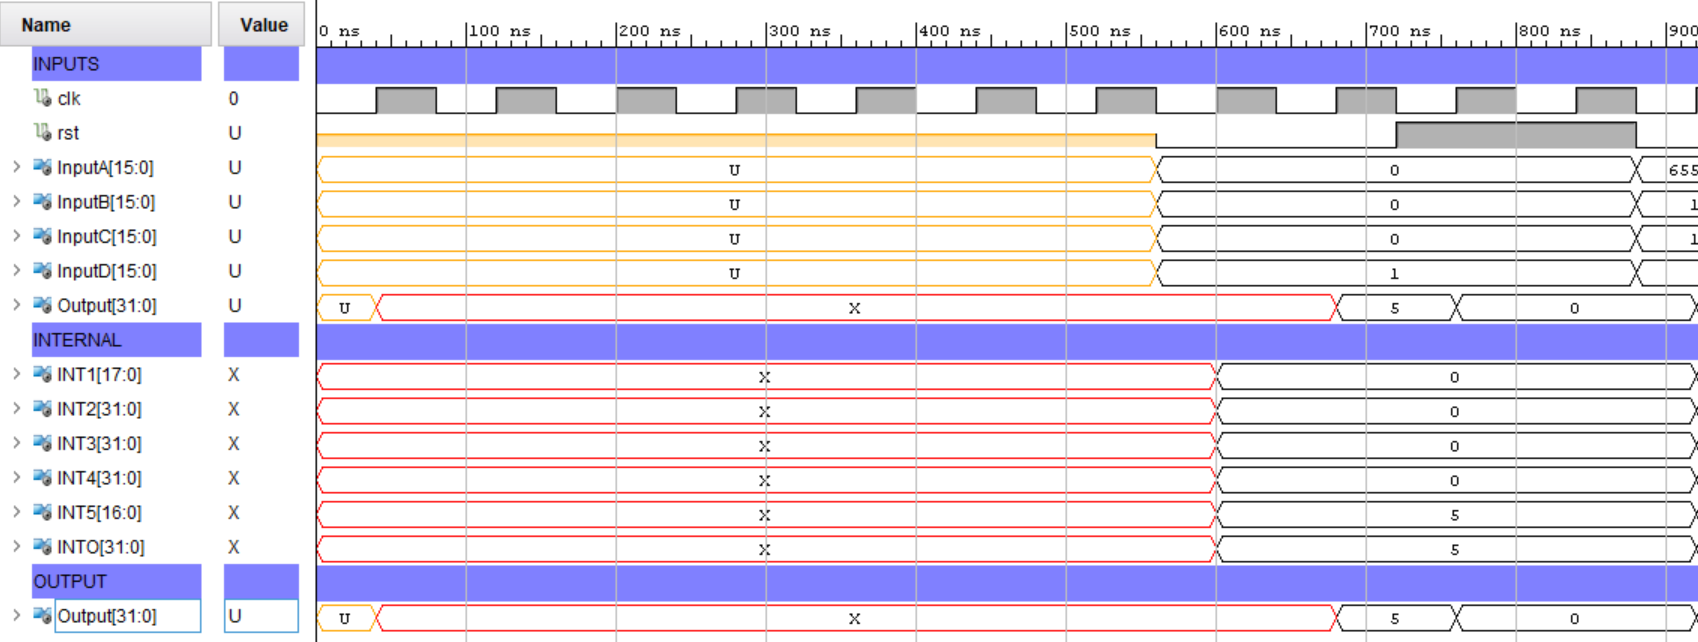
\includegraphics[width=\columnwidth]{Assets/2.1.1_waveform-initial-reset.png}
\end{figure}

\subsection*{Waveform 2: Test Sequence}
\begin{figure}[H]
    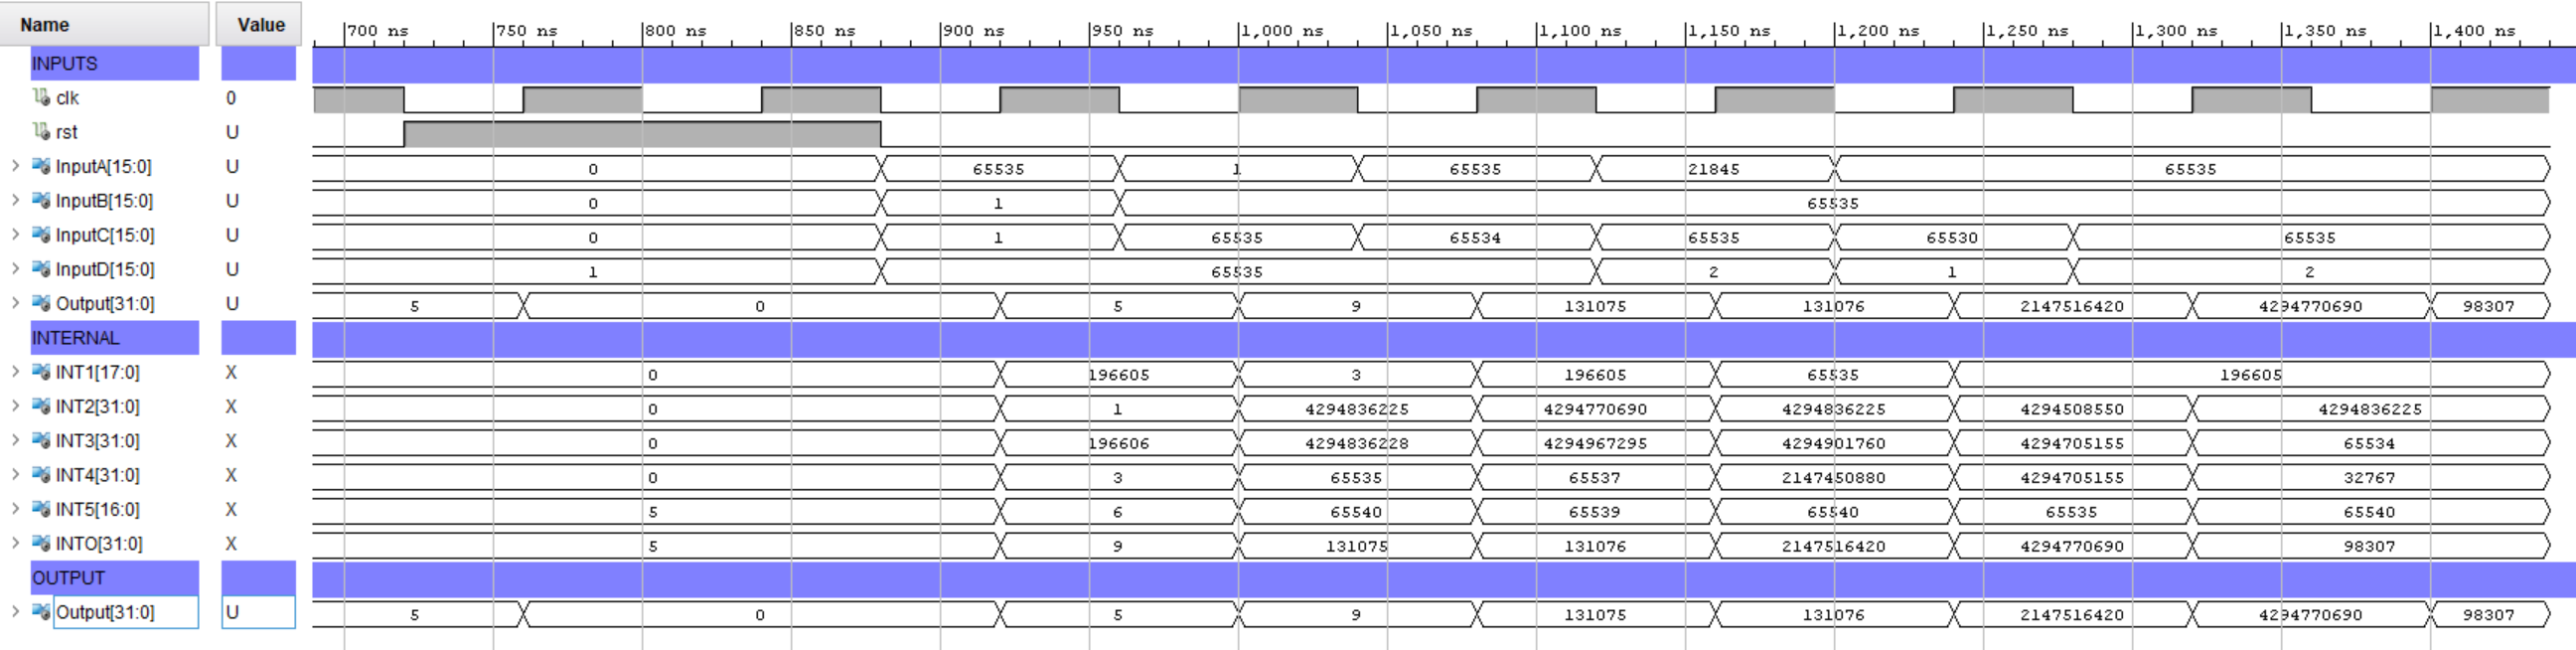
\includegraphics[width=\columnwidth]{Assets/2.1.1_waveform-test-sequence.png}
\end{figure}

\subsection*{Console Output}
\begin{figure}[H]
    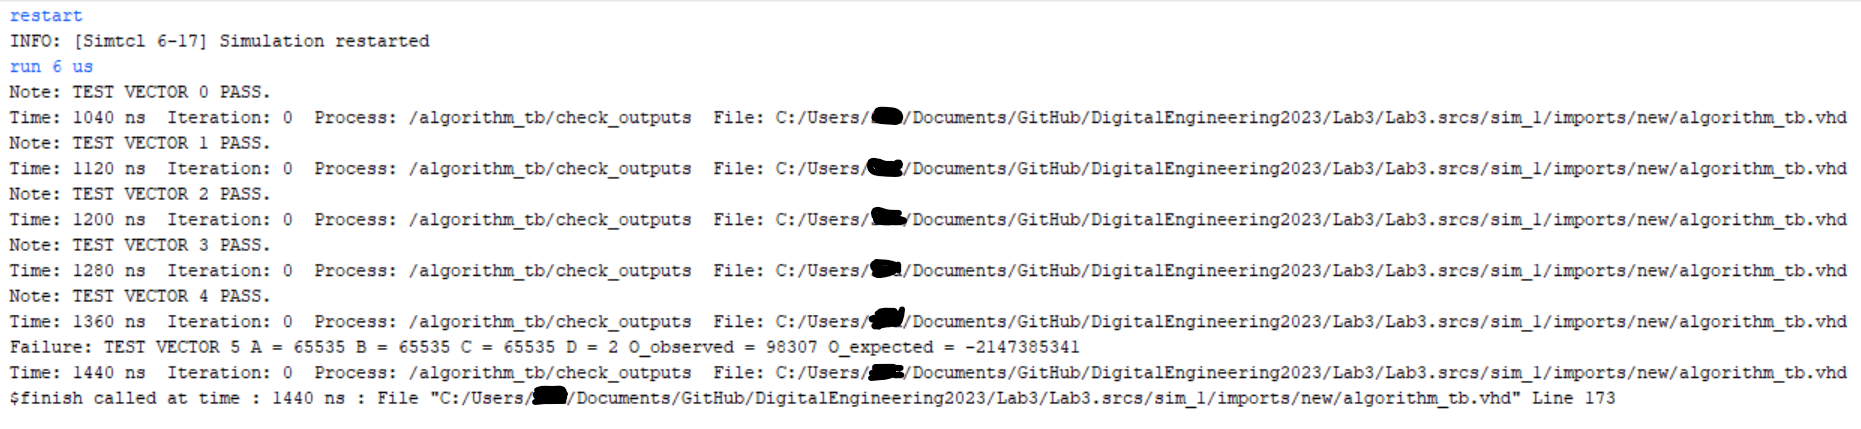
\includegraphics[width=\columnwidth]{Assets/2.1.1_console.png}
\end{figure}

\section*{2.1.2 Design Runs}
\begin{figure}[H]
    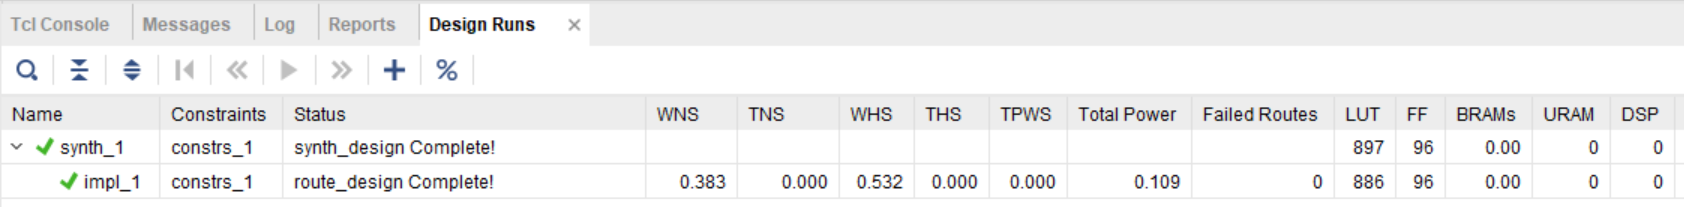
\includegraphics[width=\columnwidth]{Assets/2.1.2_design-runs.png}
\end{figure}
The best period where the constraints are met is at 107ns with a WNS of 0.383ns. The tools fail with a 106ns constraint. The fastest frequency at which this design can run, taking into account the WNS value, is 9.379MHz.


\section*{2.1.3 Post-Route Timing Report: Max Delay Path}
\begin{figure}[H]
    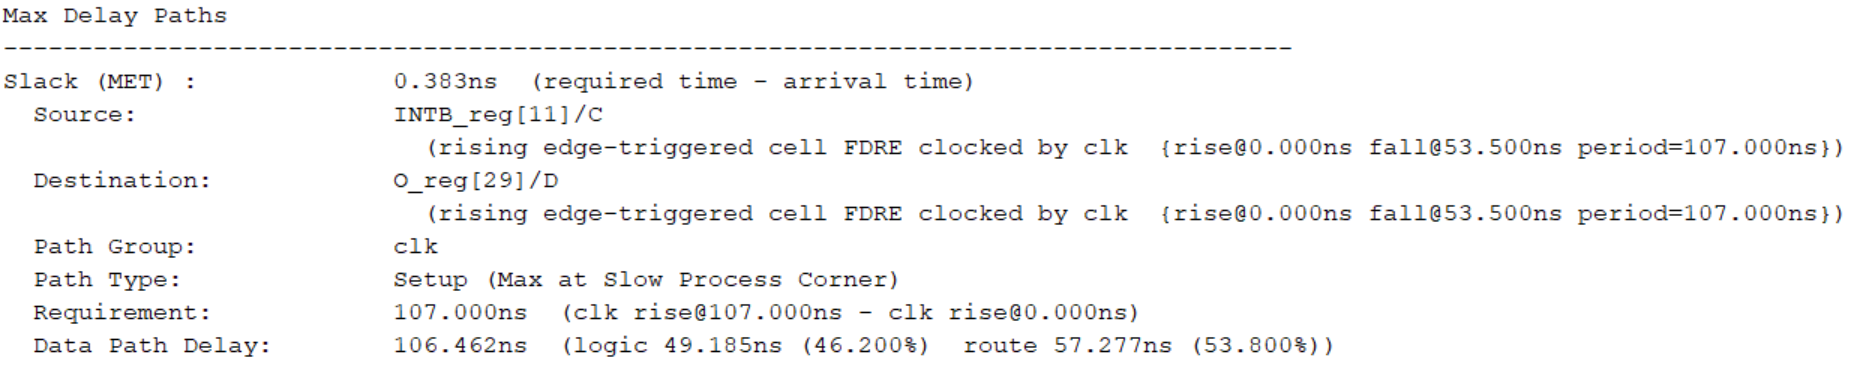
\includegraphics[width=\columnwidth]{Assets/2.1.3_max-delay-path.png}
\end{figure}

\section*{2.1.4 Pipeline 1 Behavioural Simulation}
\subsection*{Waveform 1: Global Initialisation/Reset}
\begin{figure}[H]
    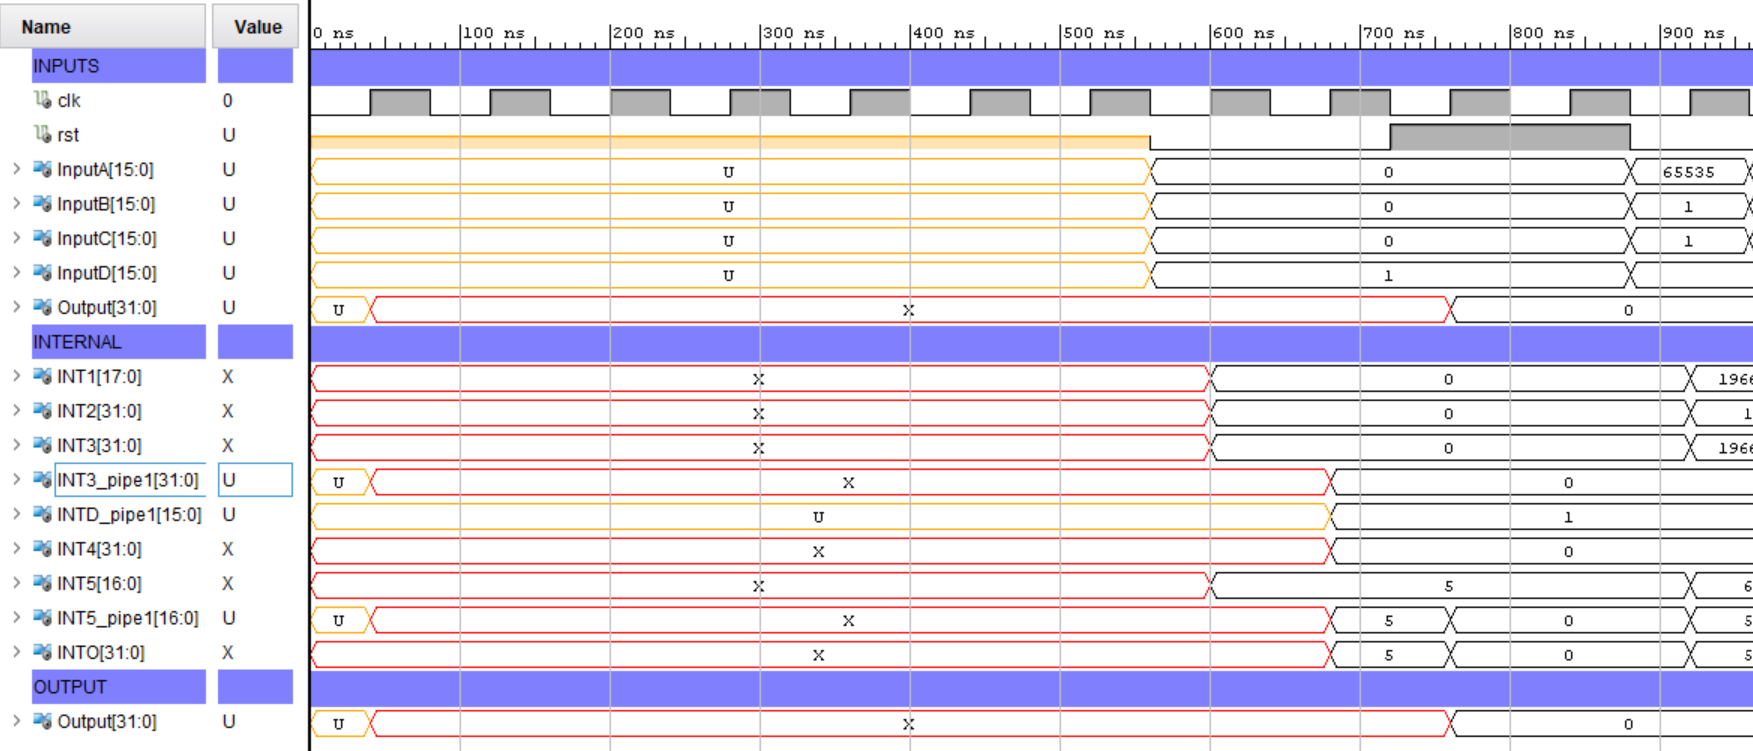
\includegraphics[width=\columnwidth]{Assets/2.1.4_waveform-initial-reset.png}
\end{figure}

\subsection*{Waveform 2: Test Sequence}
\begin{figure}[H]
    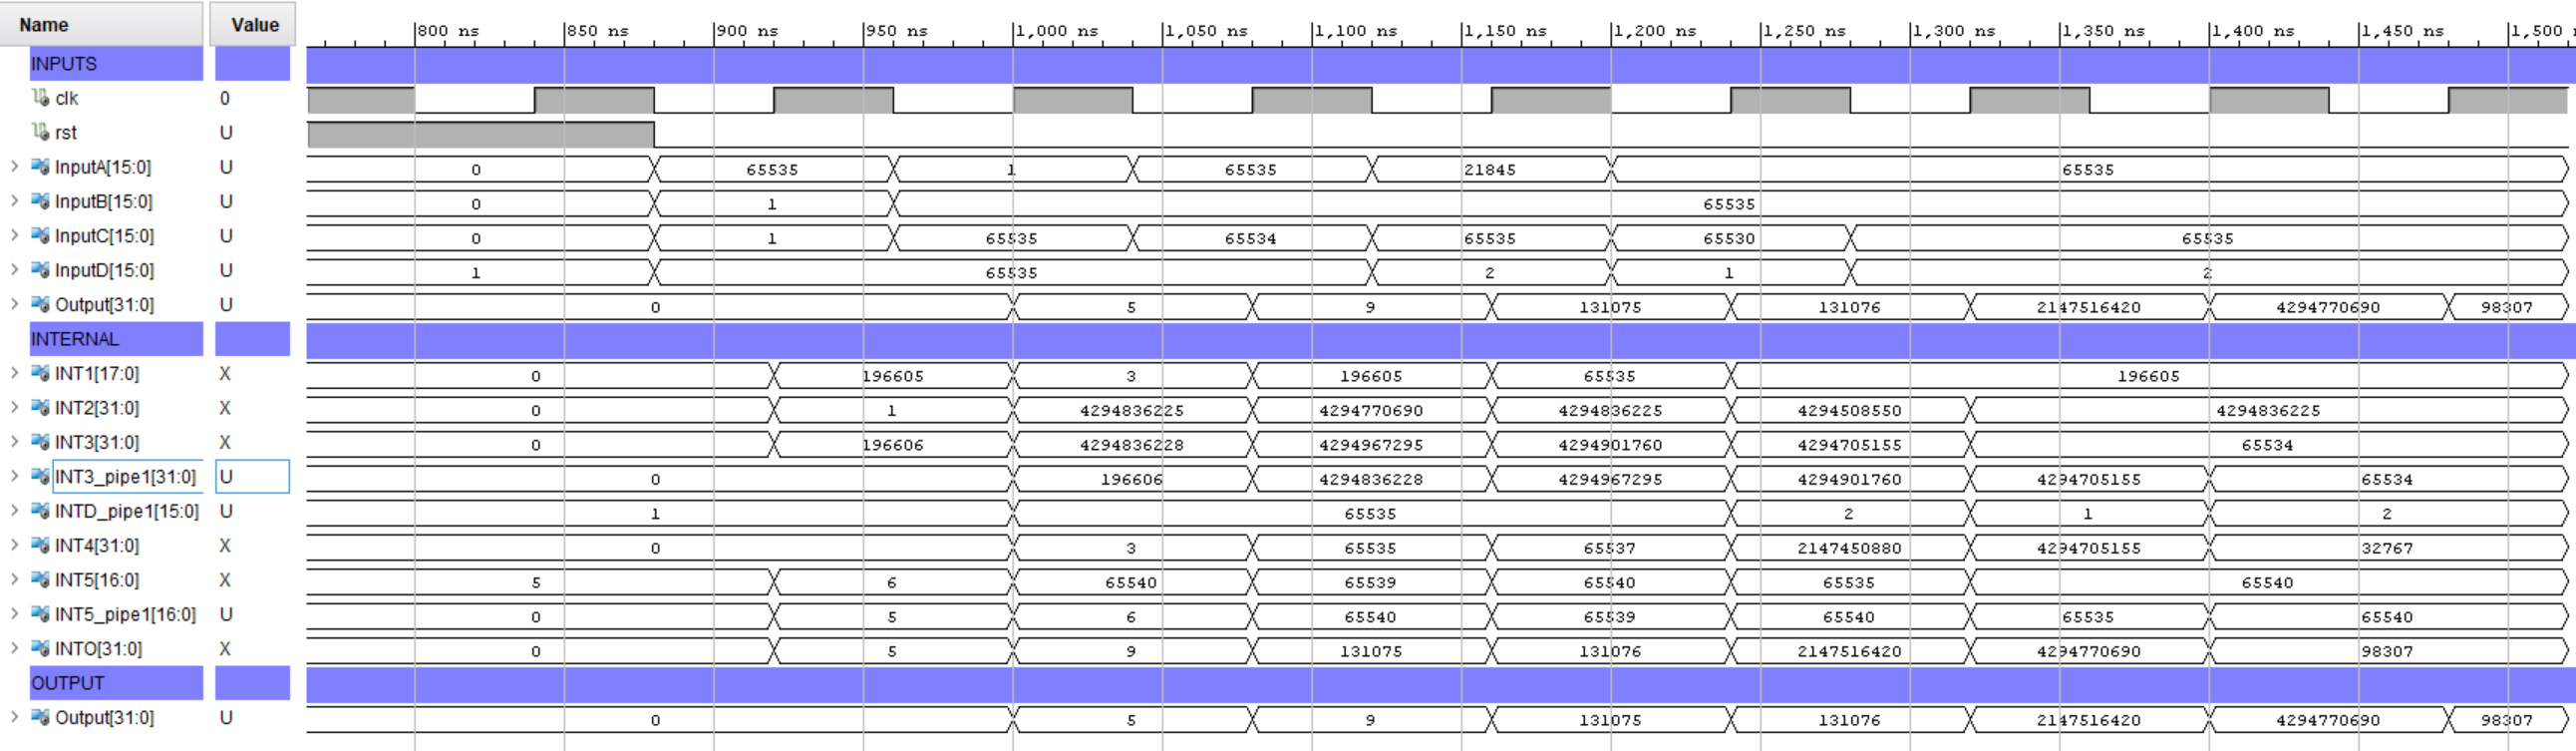
\includegraphics[width=\columnwidth]{Assets/2.1.4_waveform-test-sequence.png}
\end{figure}

\subsection*{Console}
\begin{figure}[H]
    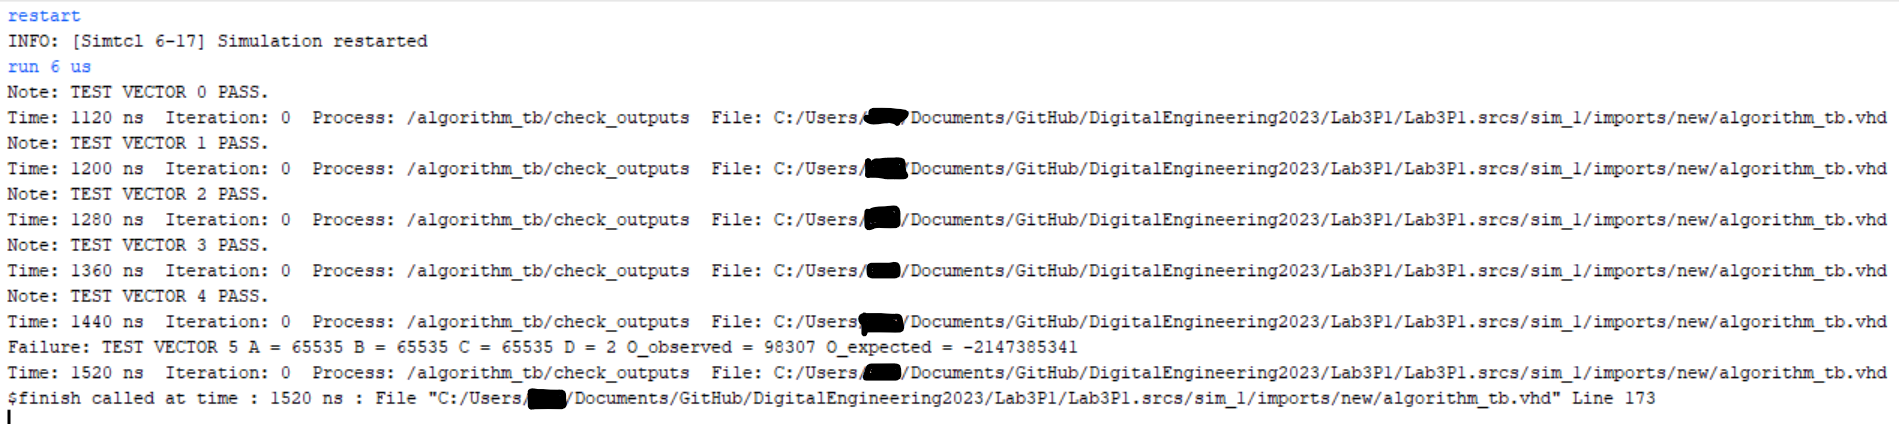
\includegraphics[width=\columnwidth]{Assets/2.1.4_console.png}
\end{figure}

\section*{2.1.5 Design Runs}
\begin{figure}[H]
    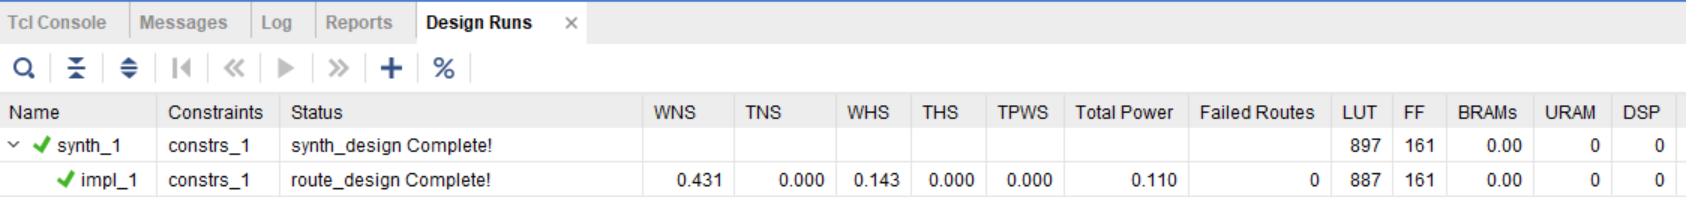
\includegraphics[width=\columnwidth]{Assets/2.1.5_design-runs.png}
\end{figure}
The best period where the constraints are met is at 96ns with a WNS of 0.431ns. The tools fail with a 95ns constraint. The fastest frequency at which this design can run, taking into account the WNS value, is 10.37MHz.

\section*{2.1.6 Post-Route Timing Report: Max Delay Path}
\begin{figure}[H]
    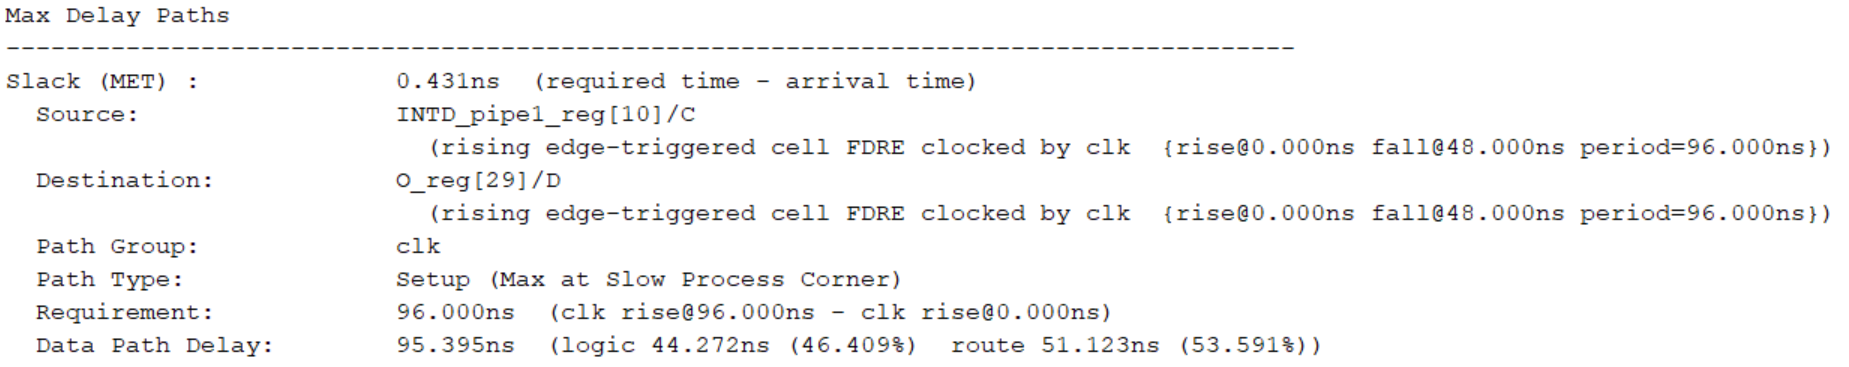
\includegraphics[width=\columnwidth]{Assets/2.1.6_max-delay-path.png}
\end{figure}
Before the pipeline was added, the critical path was detected between INTB\_reg and O\_reg. Now, we've reduced the effect of that by adding a pipeline. Now the detected critical path is between INTD\_pipe1\_reg and O\_reg. The critical path consists of the division and the addition operation, This does in fact increase the max clock period that the circuit can support as per the theory at the cost of reducing latency. The clock period we achieved in 2.1.2 was 107ns, with a pipeline stage, we can achieve 96ns.

\section*{2.1.7 Pipeline 2 Behavioural Simulation}

\subsection*{Waveform 1: Global Initialisation/Reset}
\begin{figure}[H]
    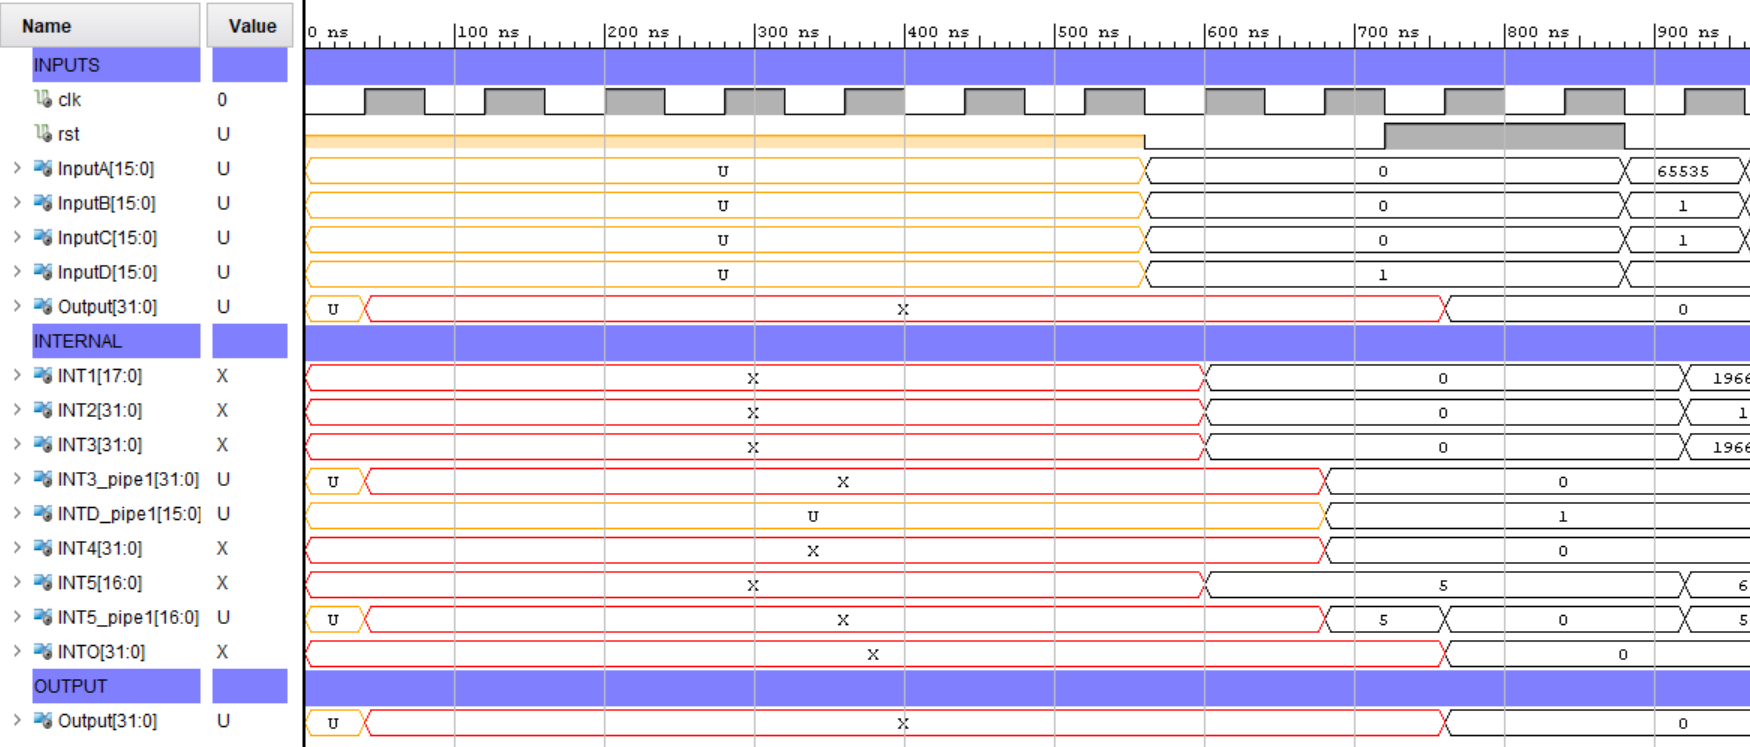
\includegraphics[width=\columnwidth]{Assets/2.1.7_waveform-initial-reset.png}
\end{figure}

\subsection*{Waveform 2: Test Sequence}
\begin{figure}[H]
    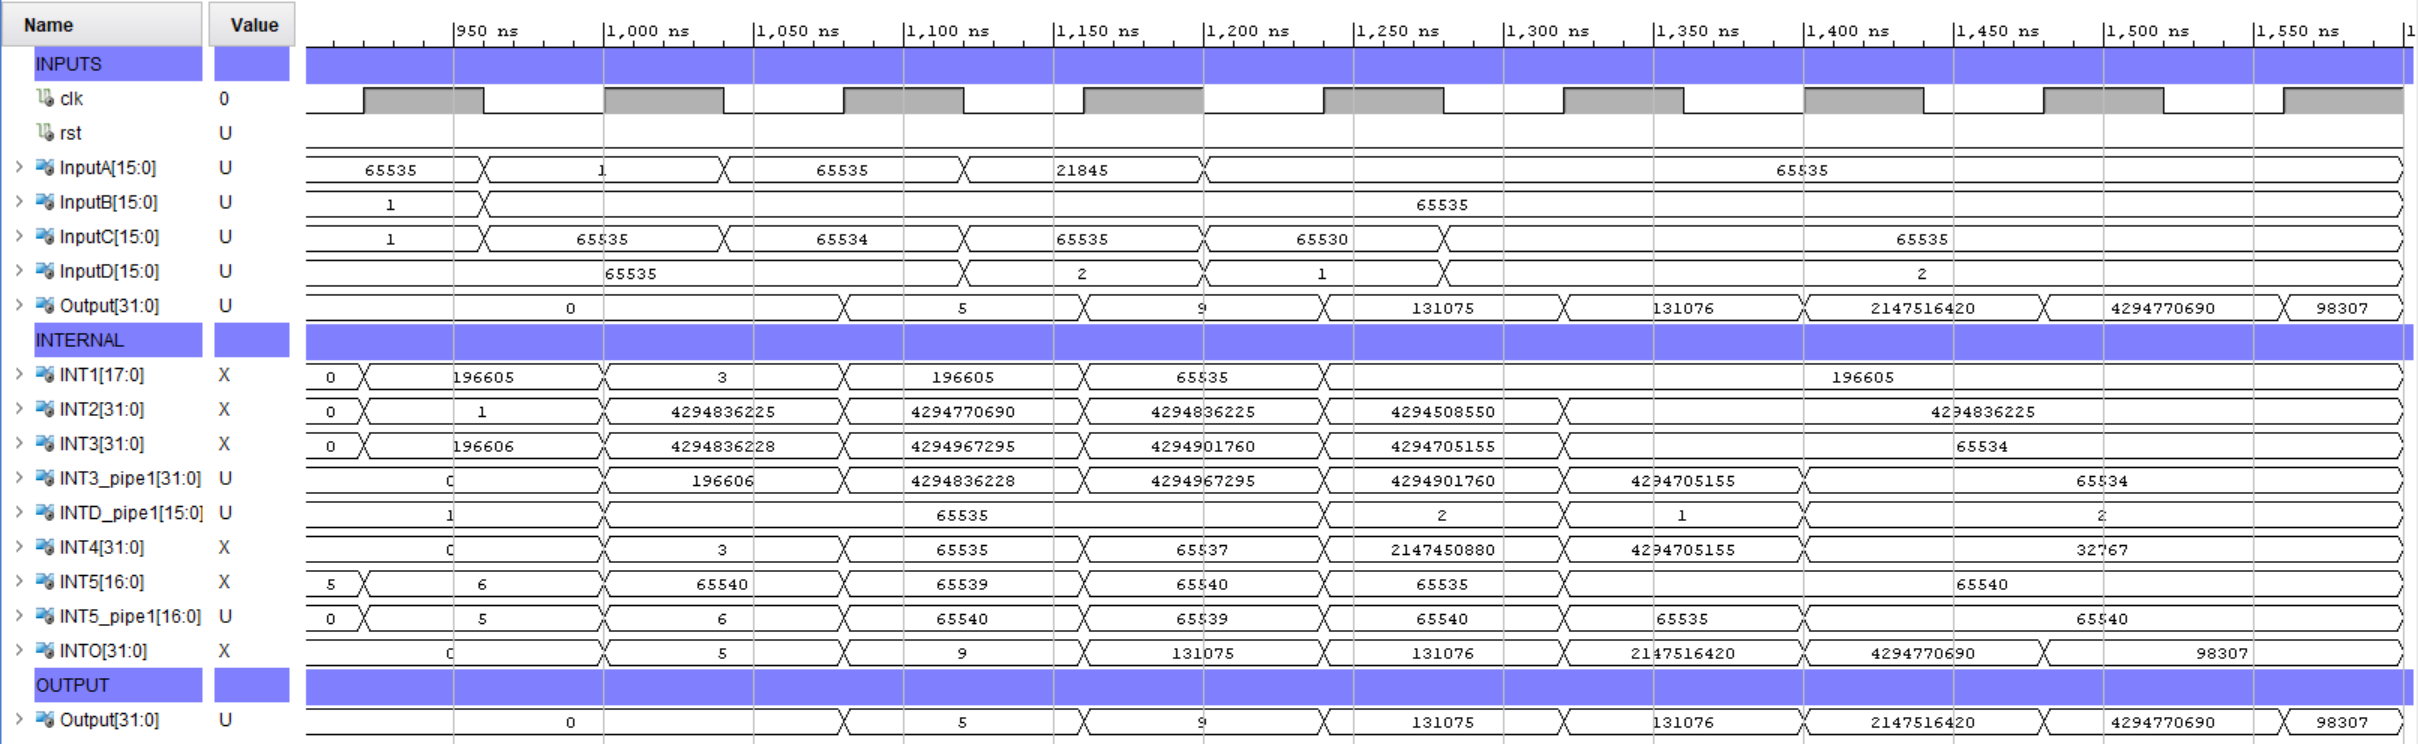
\includegraphics[width=\columnwidth]{Assets/2.1.7_waveform-test-sequence.png}
\end{figure}

\subsection*{Console}
\begin{figure}[H]
    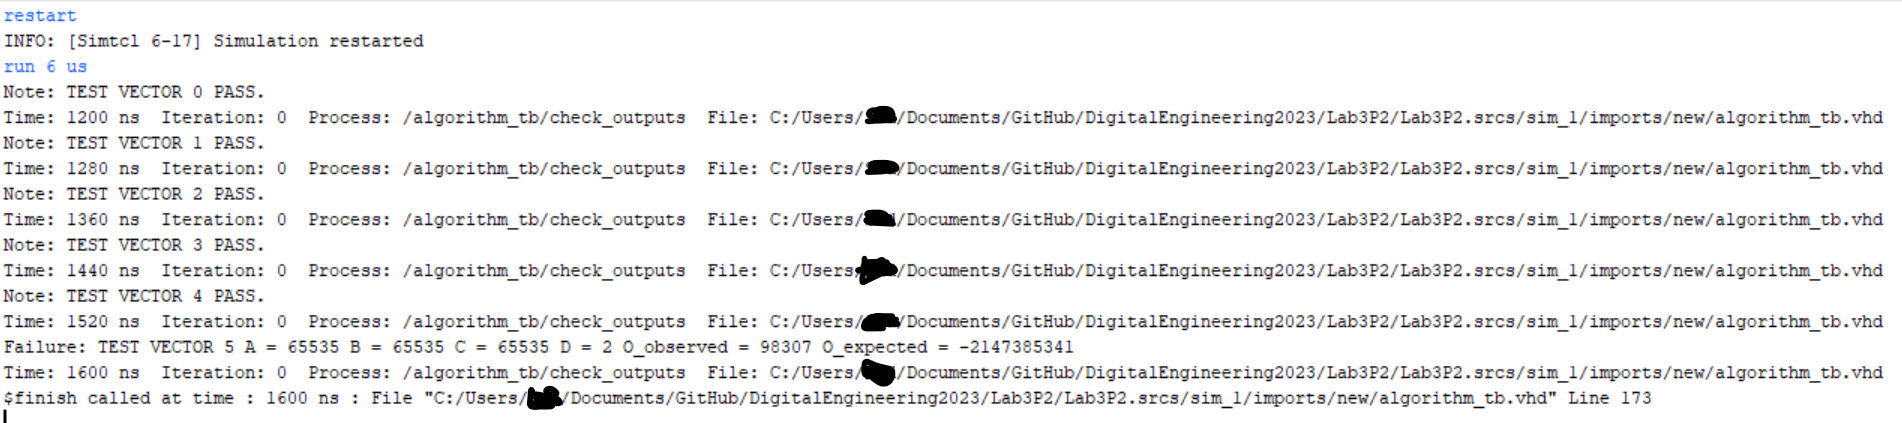
\includegraphics[width=\columnwidth]{Assets/2.1.7_console.png}
\end{figure}

\section*{2.1.8 Design Runs}
\begin{figure}[H]
    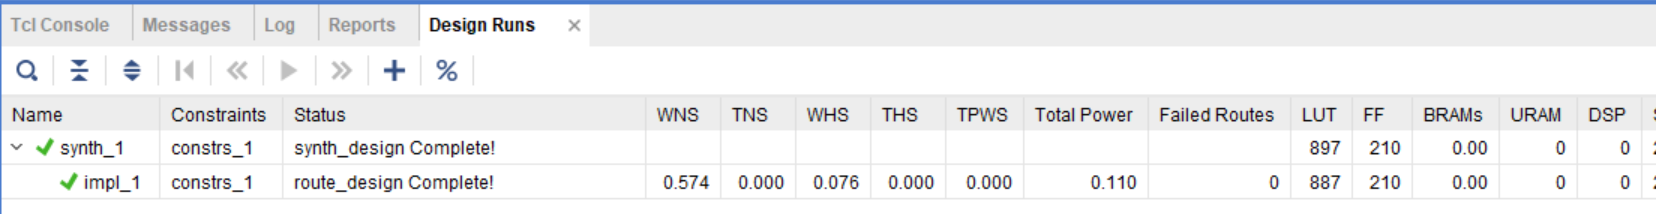
\includegraphics[width=\columnwidth]{Assets/2.1.8_design-runs.png}
\end{figure}
The best period where the constraints are met is at 90ns with a WNS of 0.574ns. The tools fail with an 89ns constraint. The fastest frequency at which this design can run, taking into account the WNS value, is 11.18MHz.

\section*{2.1.9 Post-Route Timing Report: Max Delay Path}
\begin{figure}[H]
    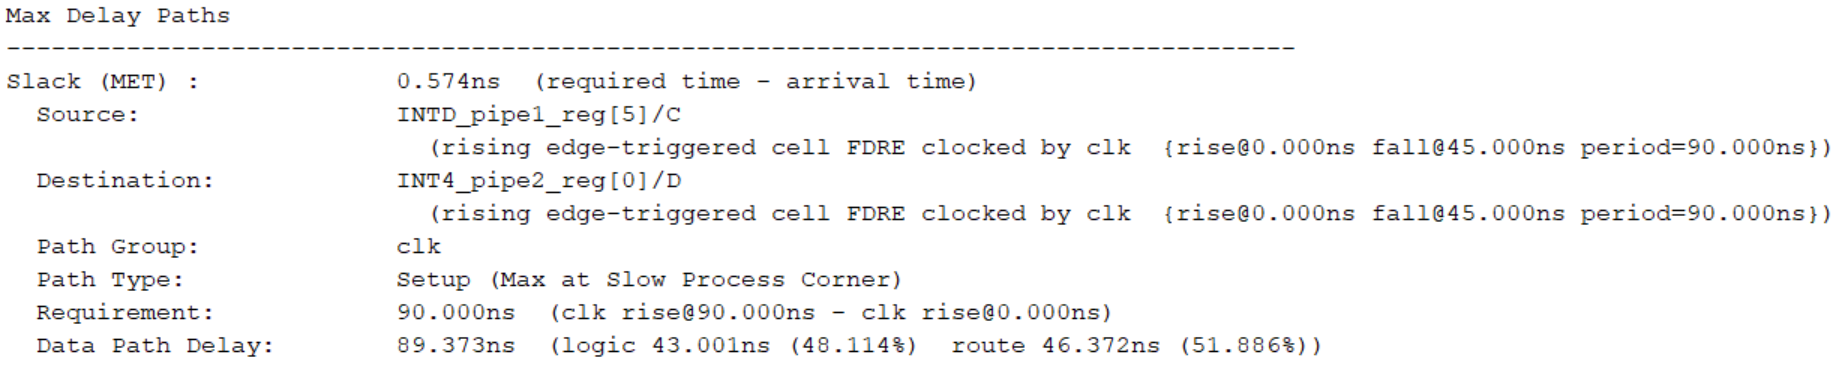
\includegraphics[width=\columnwidth]{Assets/2.1.9_max-delay-path.png}
\end{figure}
After pipeline 1 was added, the critical path was detected between INTD\_reg and O\_reg. Now, we've reduced the effect of that by adding pipeline 2. Now the detected critical path is between INTD\_pipe1\_reg and INT4\_pipe2\_reg. The critical path consists of just the division operation, This does in fact increase the max clock period that the circuit can support as per the theory at the cost of reducing latency. The clock period we achieved in 2.1.2 was 96ns, with a pipeline stage, we can achieve 90ns.

\section*{2.1.10 Behavioural Simulation}

\subsection*{Waveform 1: Global Initialisation/Reset}
\begin{figure}[H]
    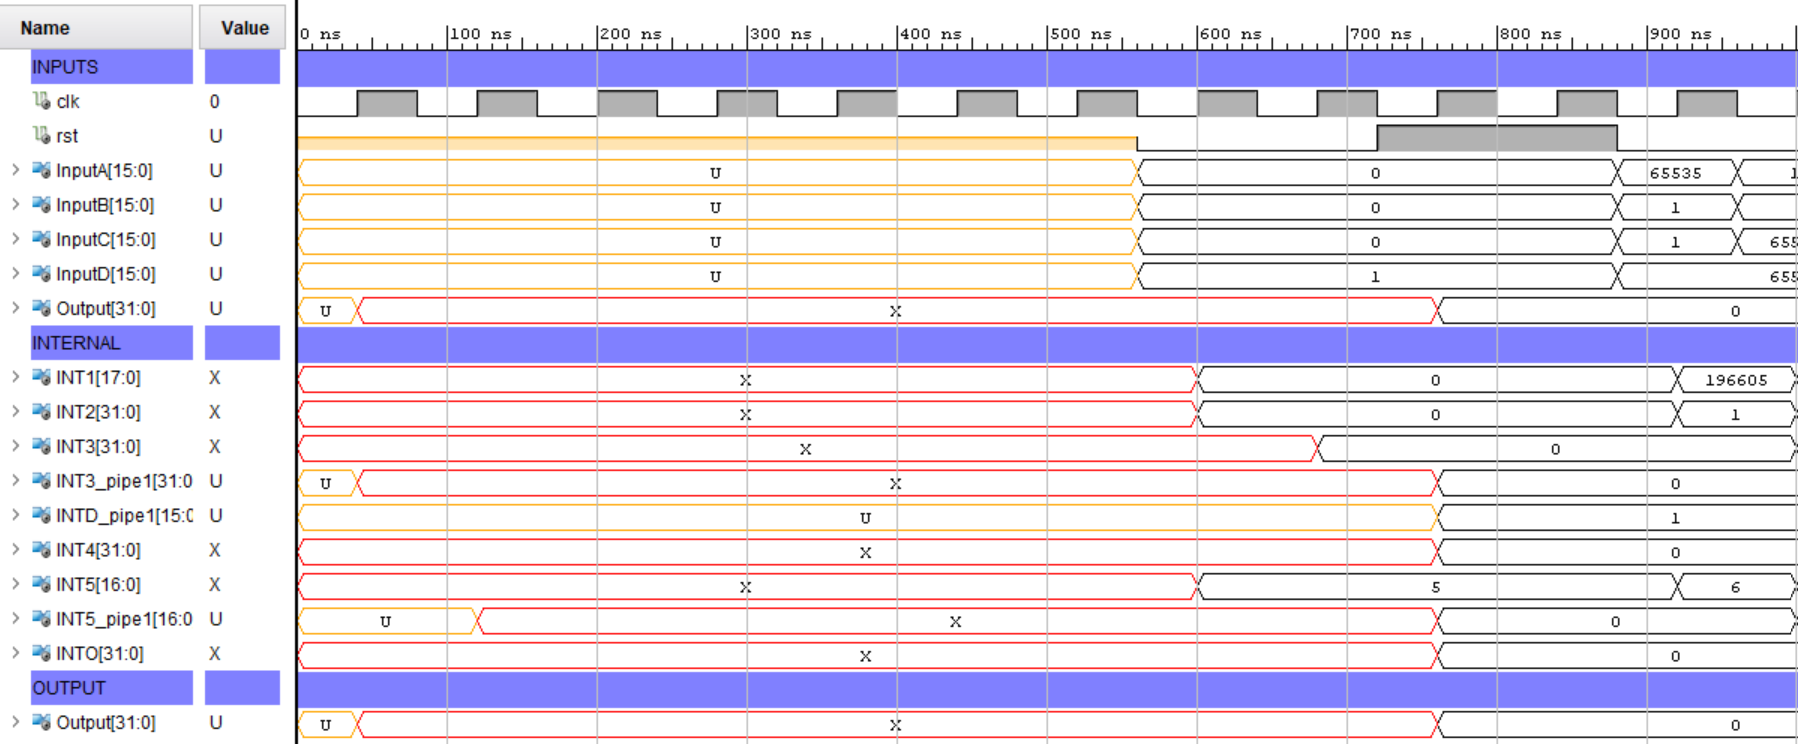
\includegraphics[width=\columnwidth]{Assets/2.1.10_waveform-initial-reset.png}
\end{figure}

\subsection*{Waveform 2: Test Sequence}
\begin{figure}[H]
    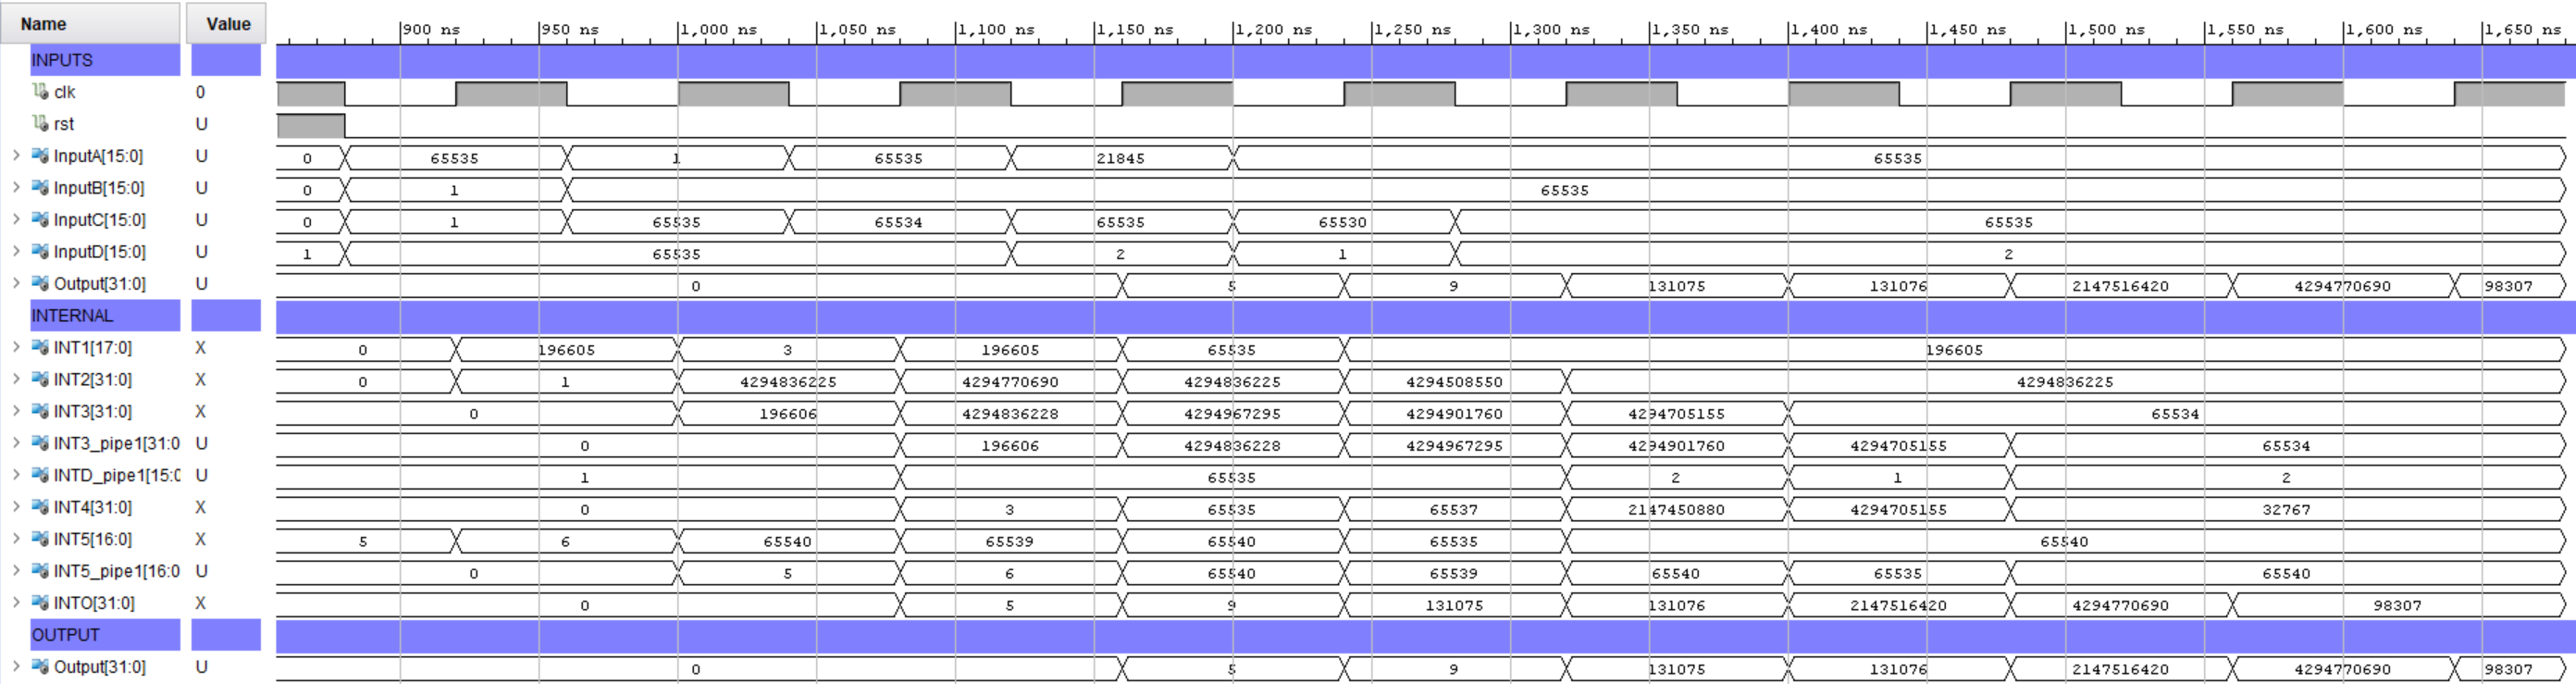
\includegraphics[width=\columnwidth]{Assets/2.1.10_waveform-test-sequence.png}
\end{figure}

\subsection*{Console}
\begin{figure}[H]
    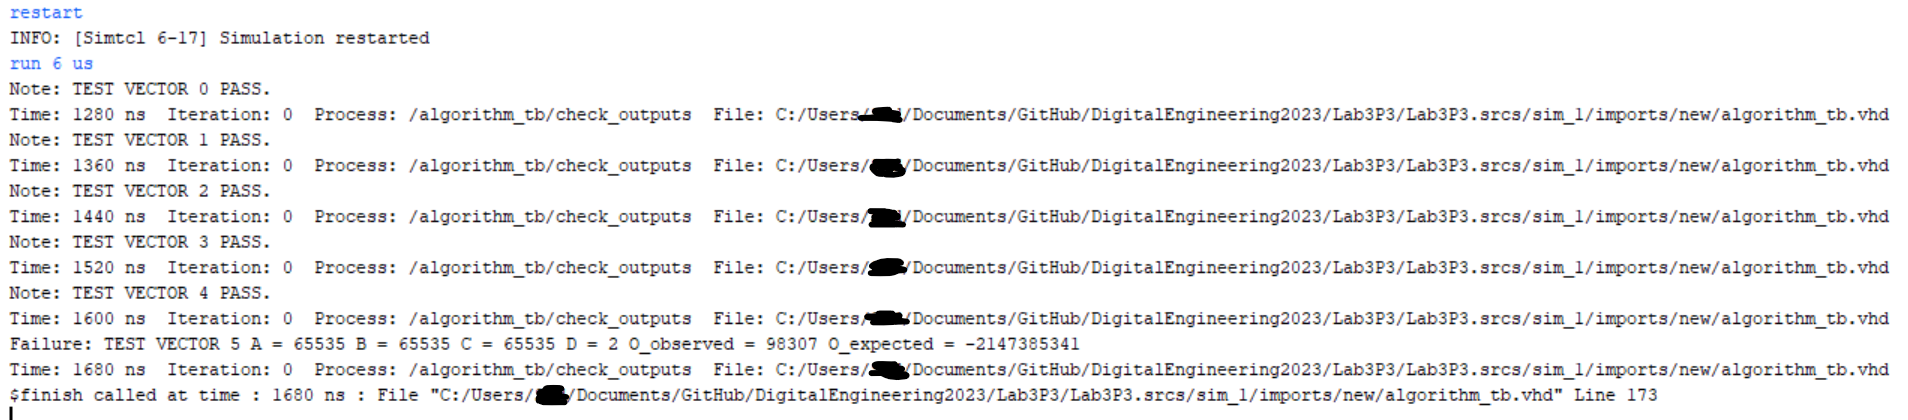
\includegraphics[width=\columnwidth]{Assets/2.1.10_console.png}
\end{figure}

\section*{2.1.11 Design Runs}
\begin{figure}[H]
    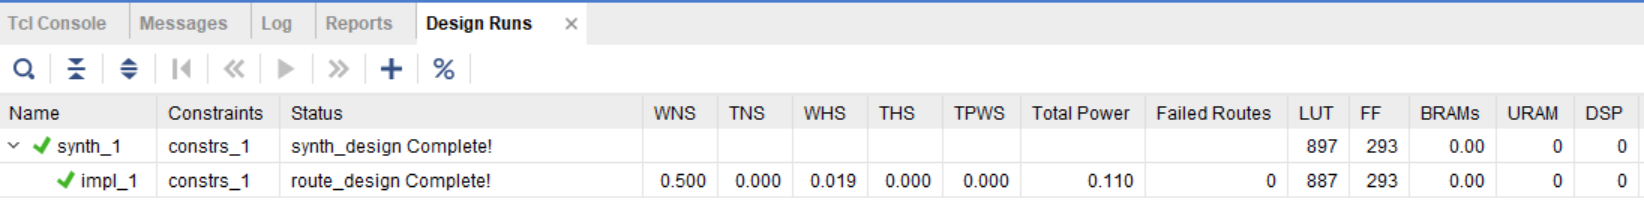
\includegraphics[width=\columnwidth]{Assets/2.1.11_design-runs.png}
\end{figure}
The best period where the constraints are met is at 90ns with a WNS of 0.5ns. The tools fail with an 89ns constraint. The fastest frequency at which this design can run, taking into account the WNS value, is 11.17MHz.

\section*{2.1.12 Post-Route Timing Report: Max Delay Path}
\begin{figure}[H]
    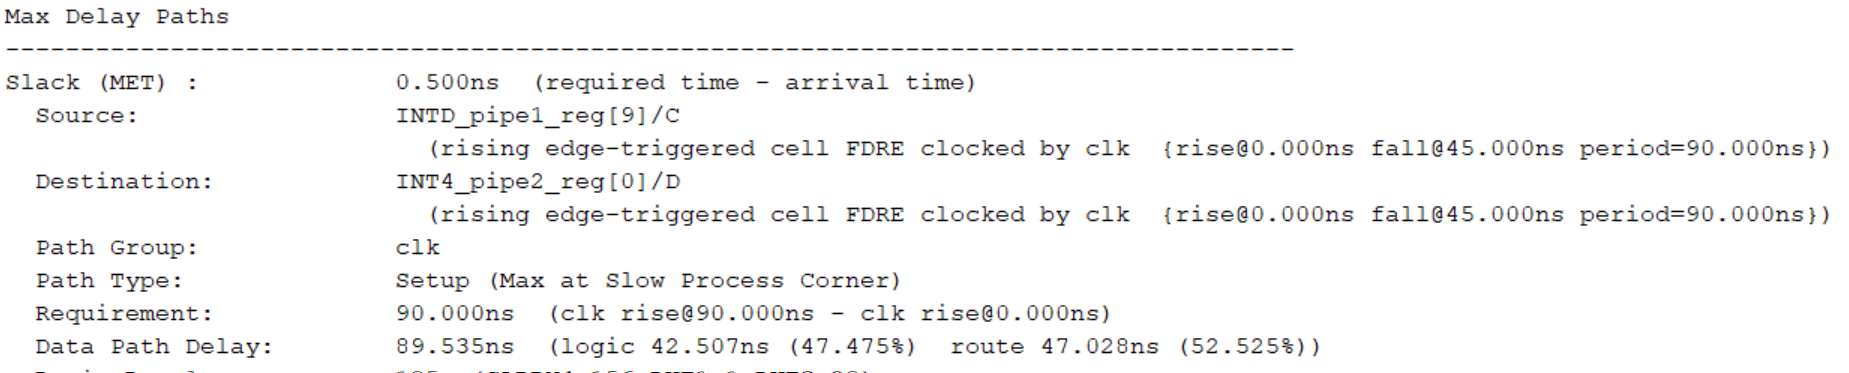
\includegraphics[width=\columnwidth]{Assets/2.1.12_max-path-delays.png}
\end{figure}
After pipeline 2 was added, the critical path was detected between INTD\_pipe1\_reg and INT4\_pipe2\_reg. Since adding the third pipeline, we don't see an improvement, but rather we see a decline in performance. The clock period we achieved in 2.1.2 was 90ns, with this pipeline, the clock period hasn't changed.

\chapter*{Task B: IP Components}

\section*{2.2.1 Behavioural Simulation}

\subsection*{Waveform 1: Global Initialisation/Reset}
\begin{figure}[H]
    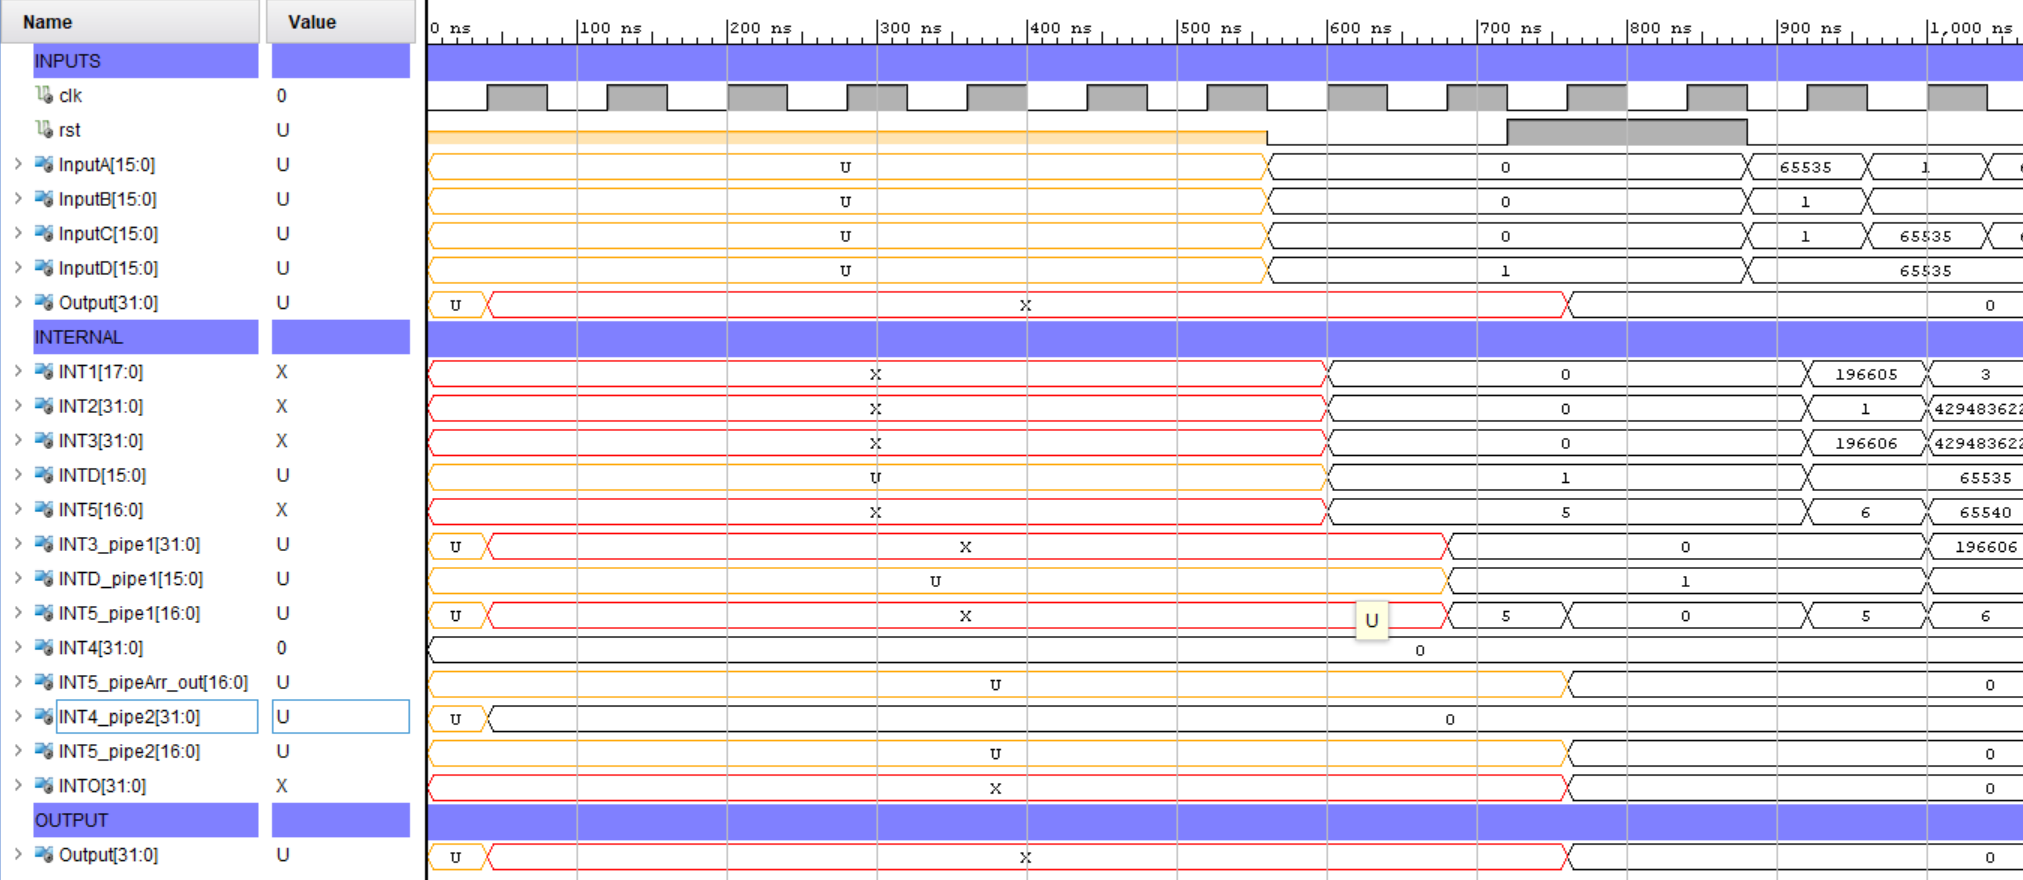
\includegraphics[width=\columnwidth]{Assets/2.2.1_waveform-initial-reset.png}
\end{figure}

\subsection*{Waveform 2: Test Sequence 1}
\begin{figure}[H]
    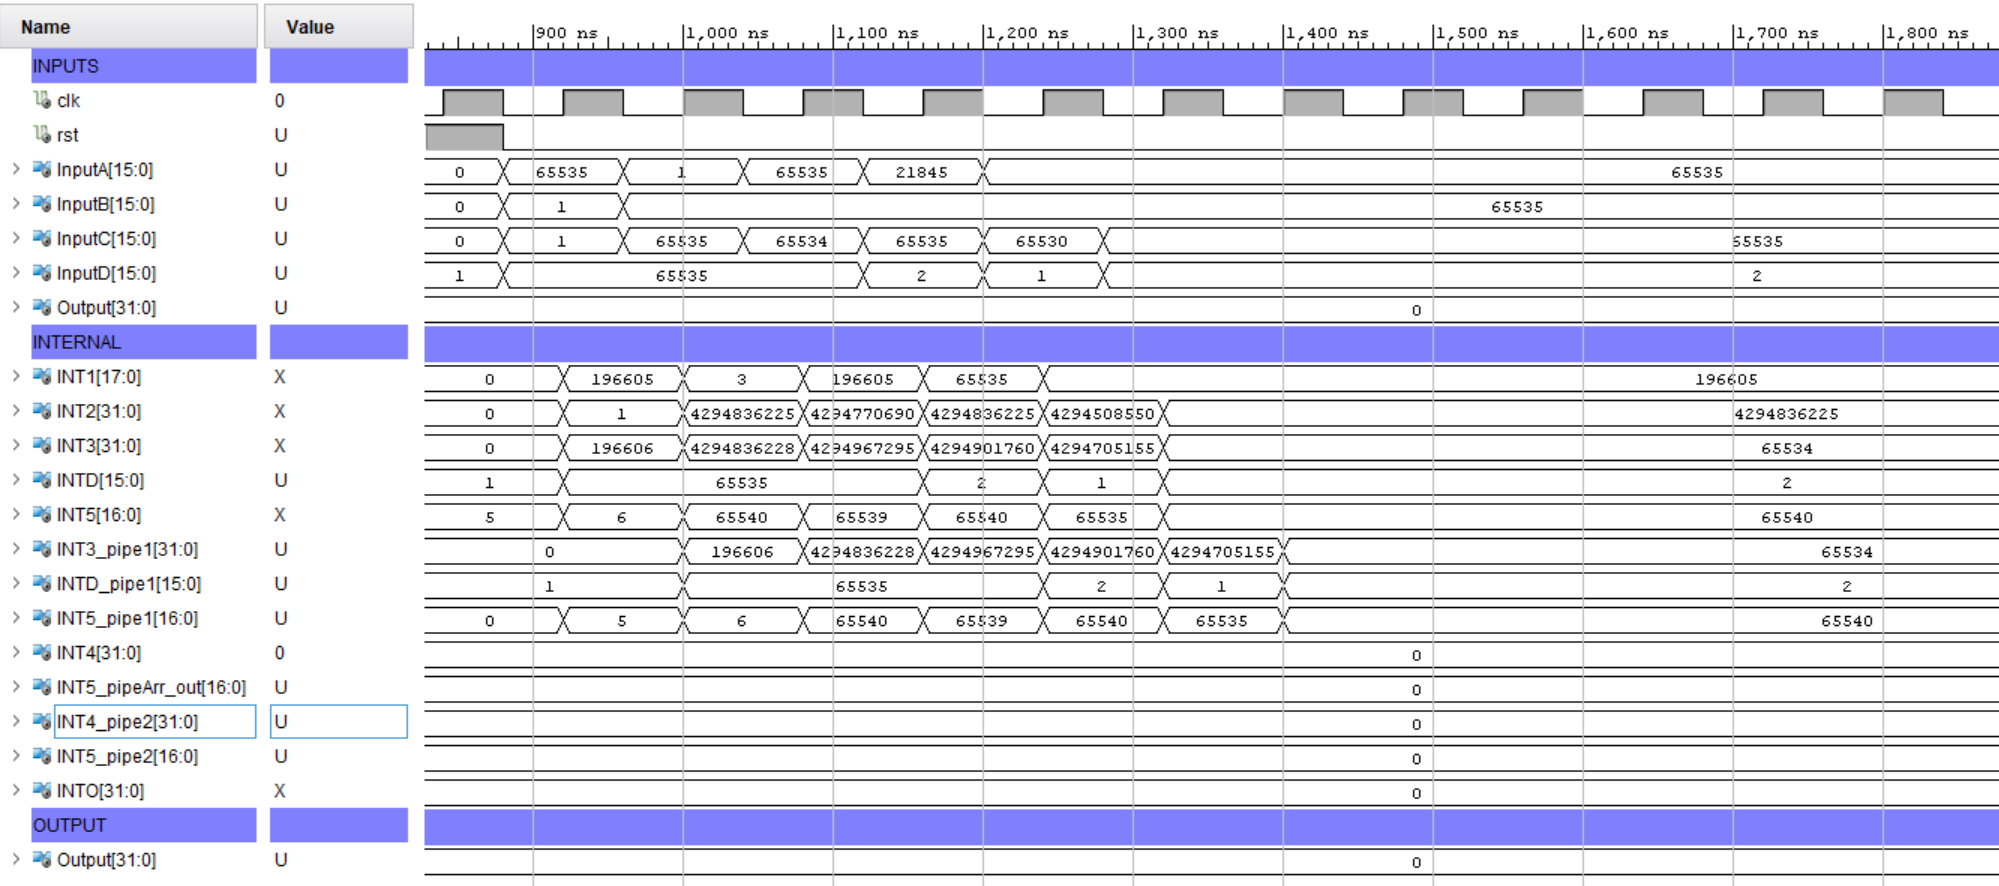
\includegraphics[width=\columnwidth]{Assets/2.2.1_waveform-test-sequence-1.png}
\end{figure}

\subsection*{Waveform 3: Test Sequence 2}
\begin{figure}[H]
    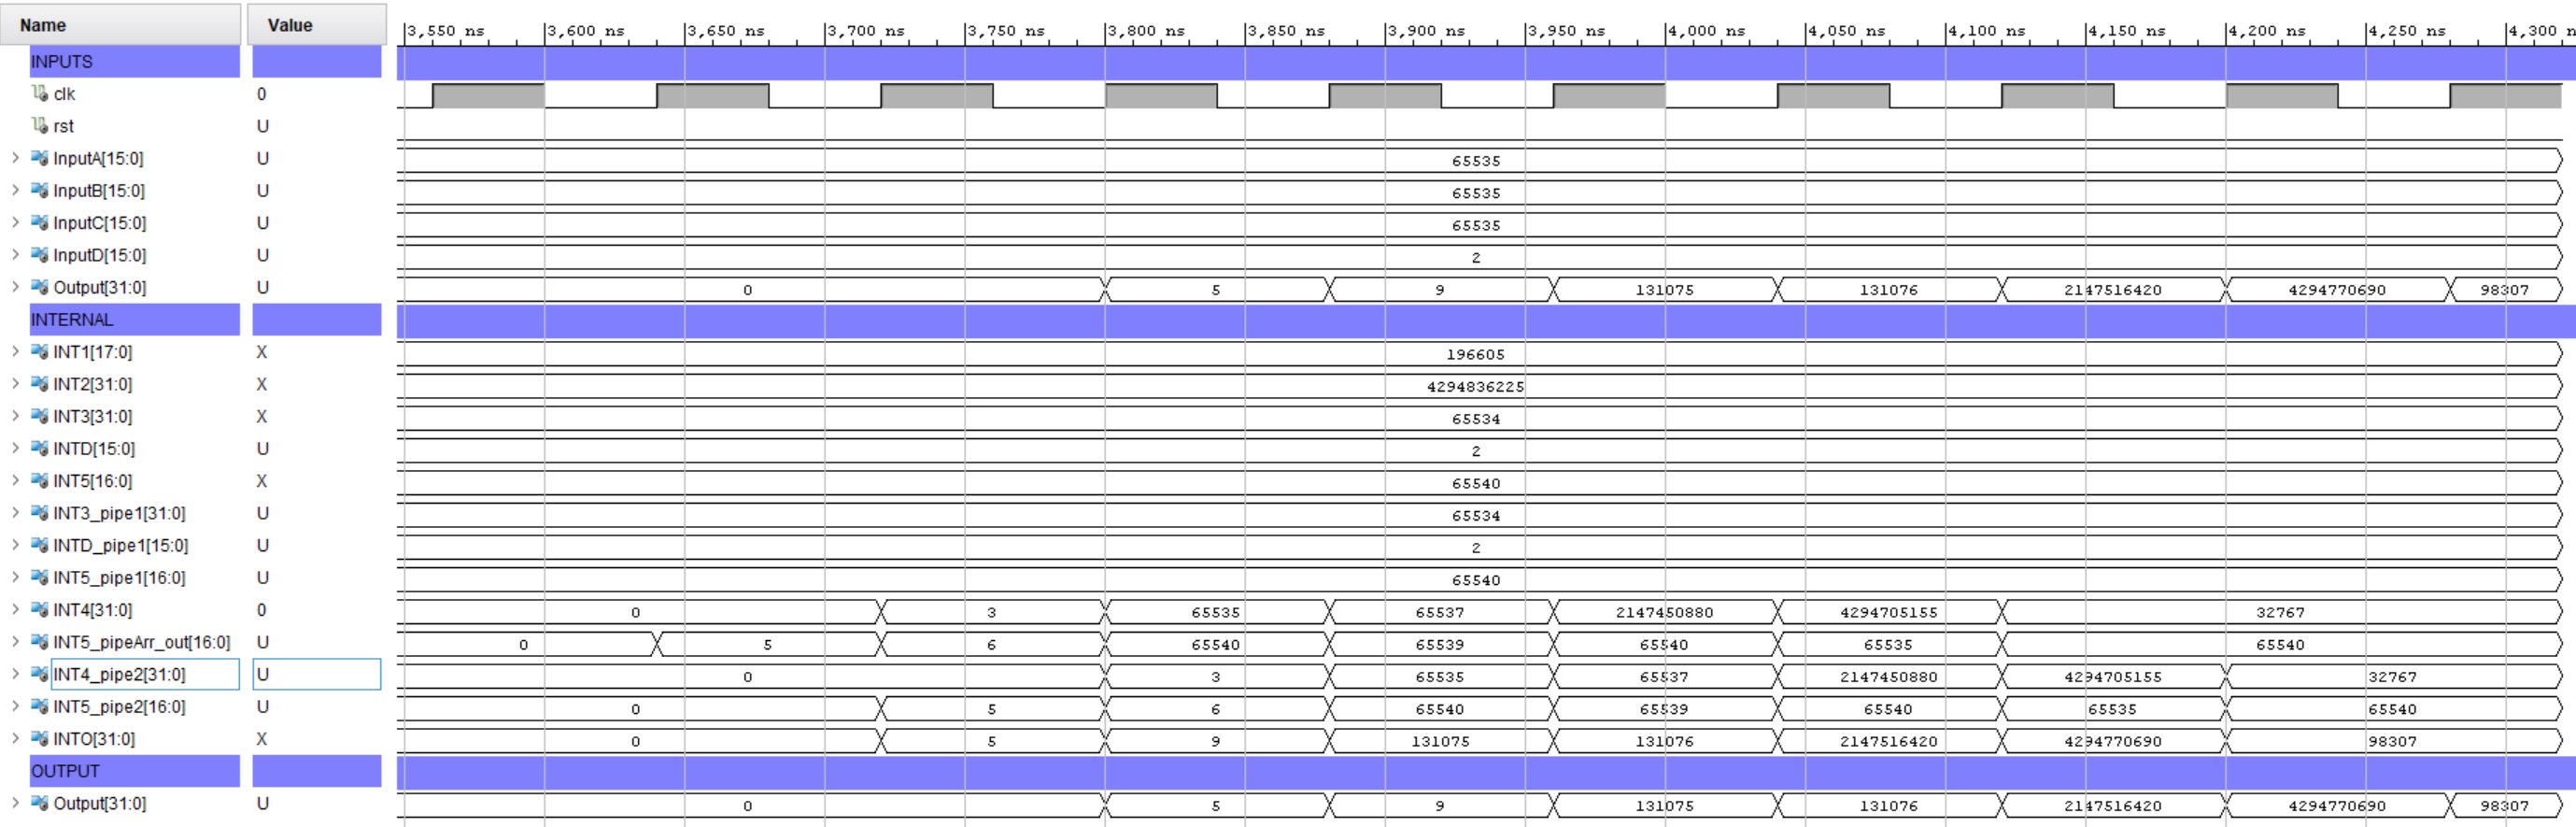
\includegraphics[width=\columnwidth]{Assets/2.2.1_waveform-test-sequence-2.png}
\end{figure}

\subsection*{Console}
\begin{figure}[H]
    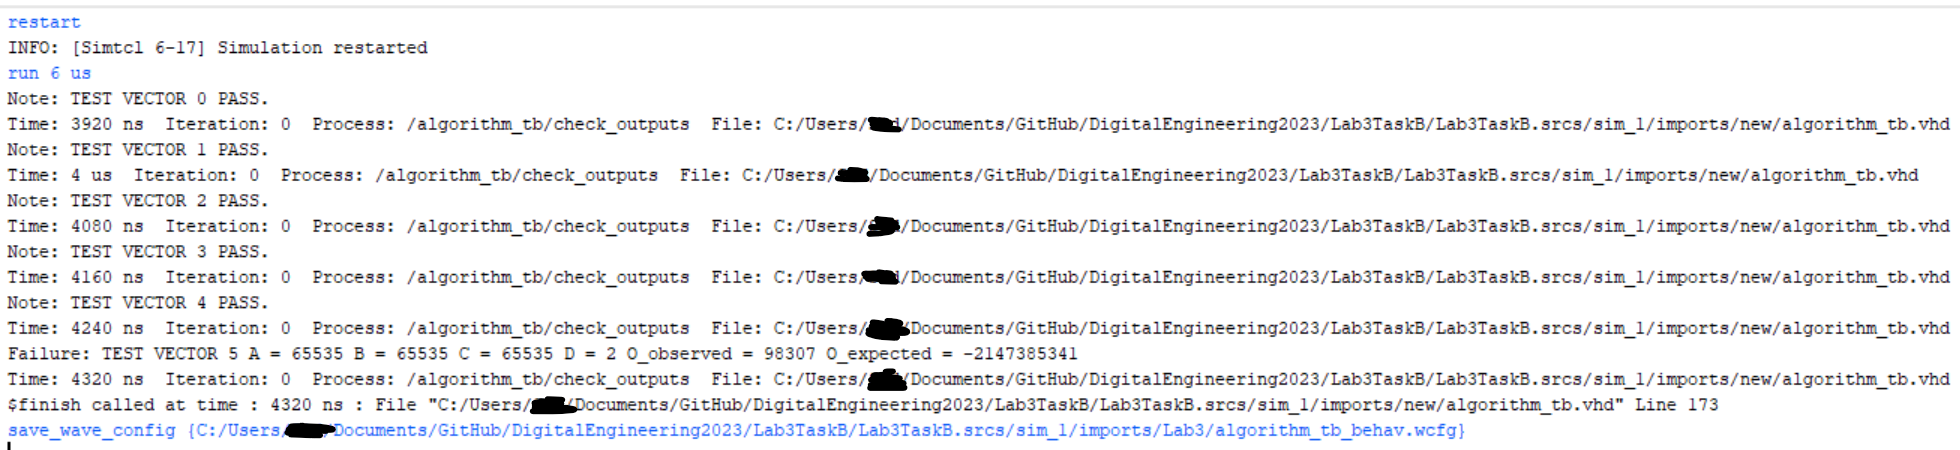
\includegraphics[width=\columnwidth]{Assets/2.2.1_console.png}
\end{figure}

\section*{2.2.2 Design Runs}
\begin{figure}[H]
    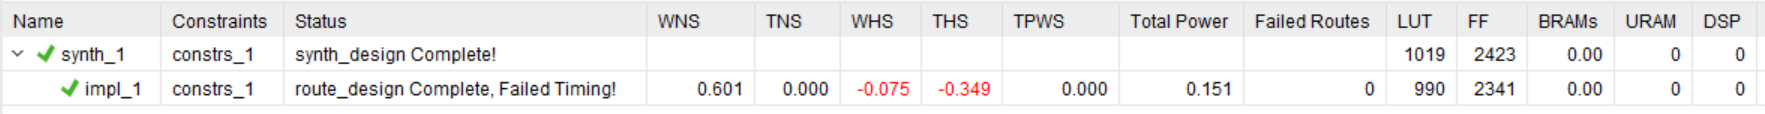
\includegraphics[width=\columnwidth]{Assets/2.2.2_design-runs.png}
\end{figure}
The best period where the constraints are met is at 14ns with a WNS of 0.601ns (a massive improvement from the 90ns max period we achieved before). The tools fail with a 13ns constraint. The fastest frequency at which this design can run, considering the WNS value, is 74.63MHz. The vast increase in flip-flops has also been noted.

\section*{2.2.3 Post-Route Timing Report: Max Delay Path}
\begin{figure}[H]
    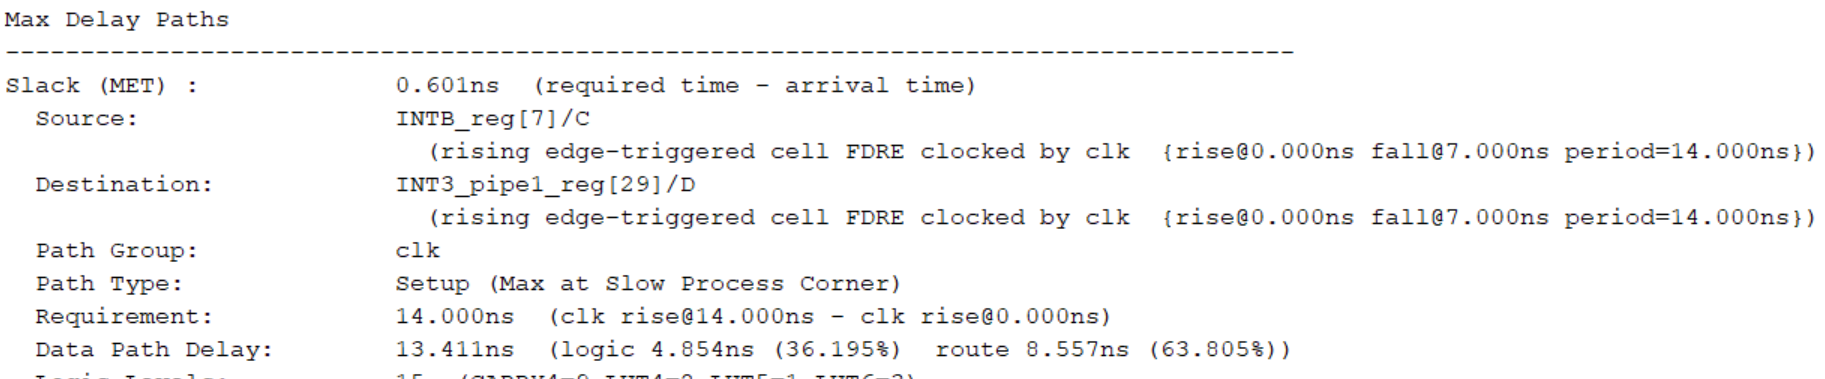
\includegraphics[width=\columnwidth]{Assets/2.2.3_max-delay-path.png}
\end{figure}
From this report, we can identify that the critical path lies between INTB\_reg and INT3\_pipe1\_reg. The two mathematical operations which lie in the critical path is the multiplication and addition, this is before the first pipeline and after the input registers.

\section*{2.2.4 Behavioural Simulation}
\subsection*{Waveform 1: Global Initialisation/Reset}
\begin{figure}[H]
    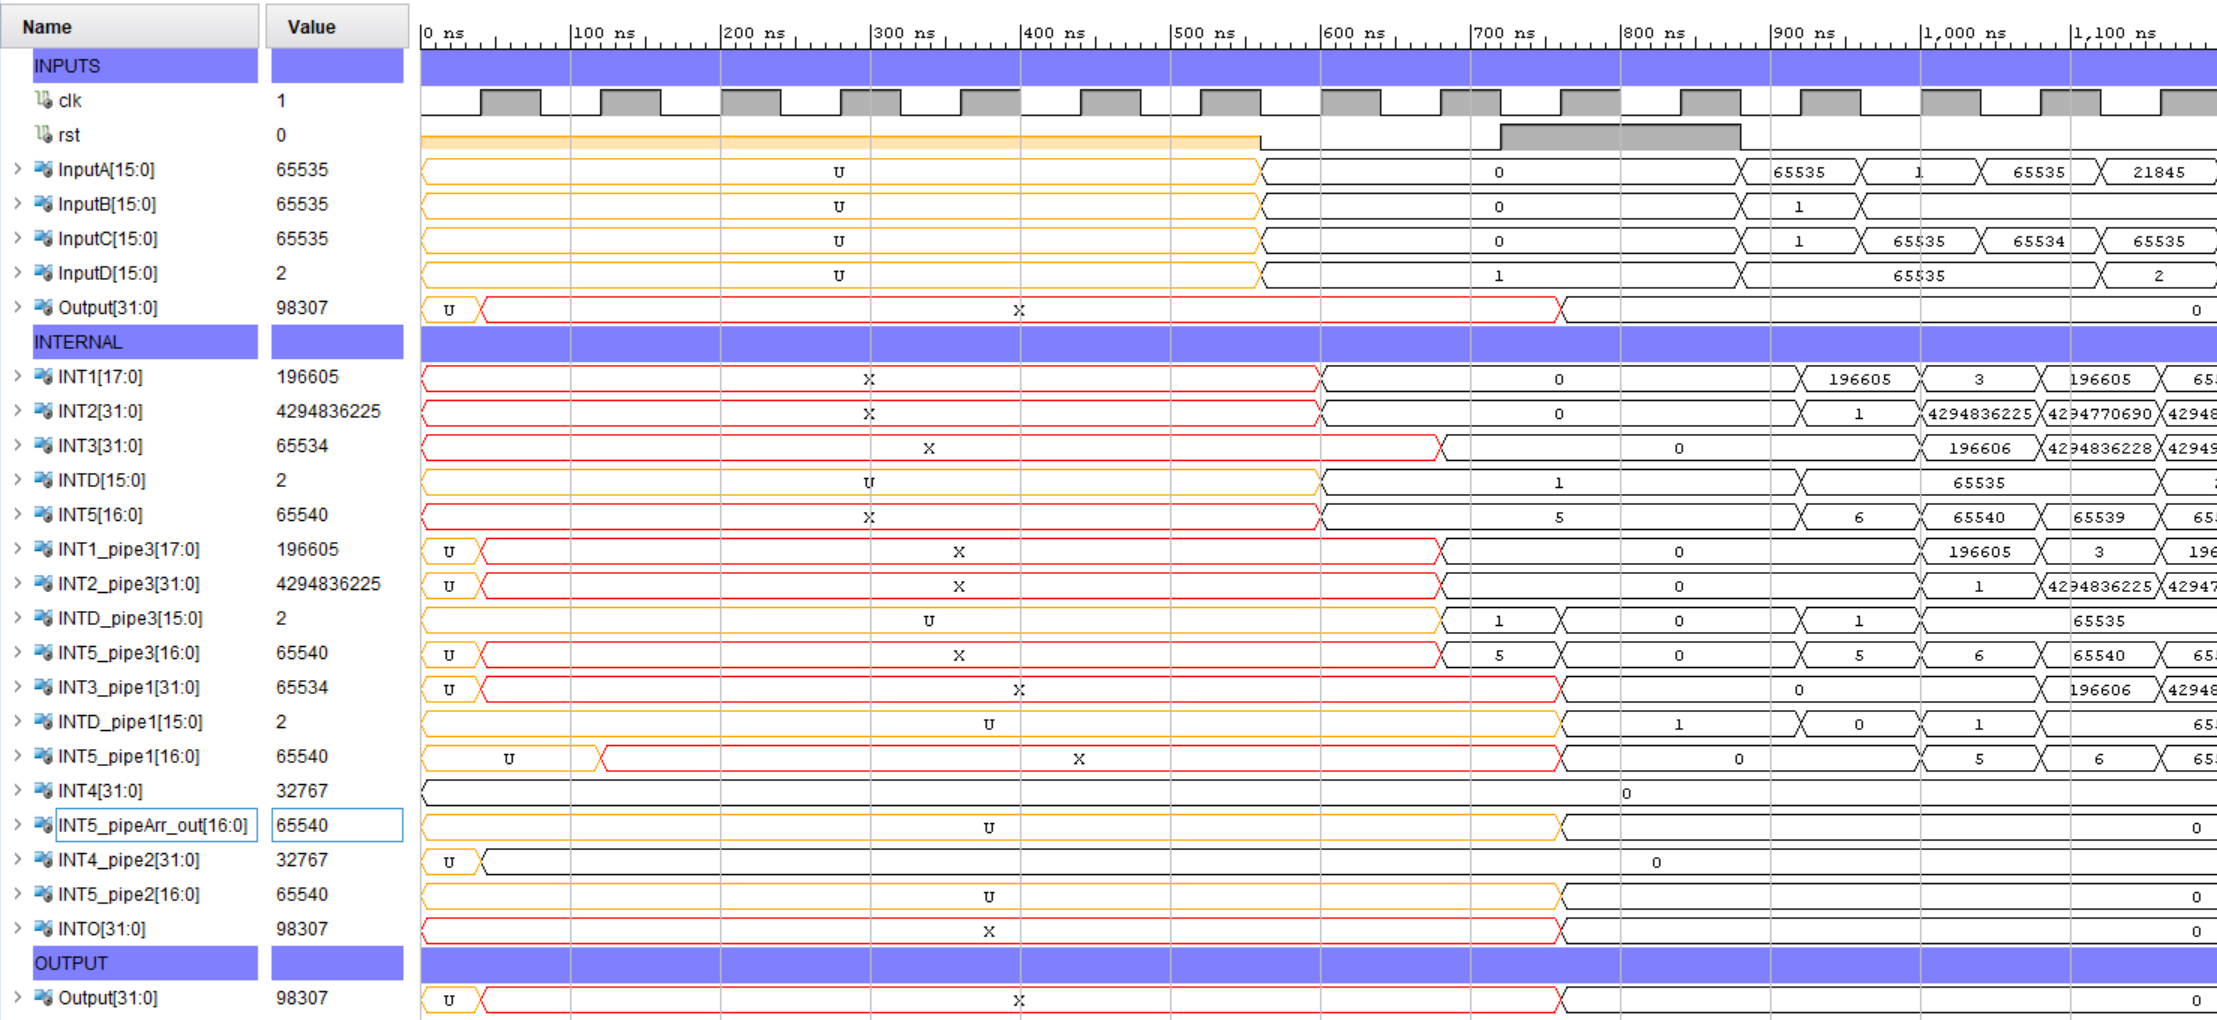
\includegraphics[width=\columnwidth]{Assets/2.2.4_waveform-initial-reset.png}
\end{figure}

\subsection*{Waveform 2: Test Sequence 1}
\begin{figure}[H]
    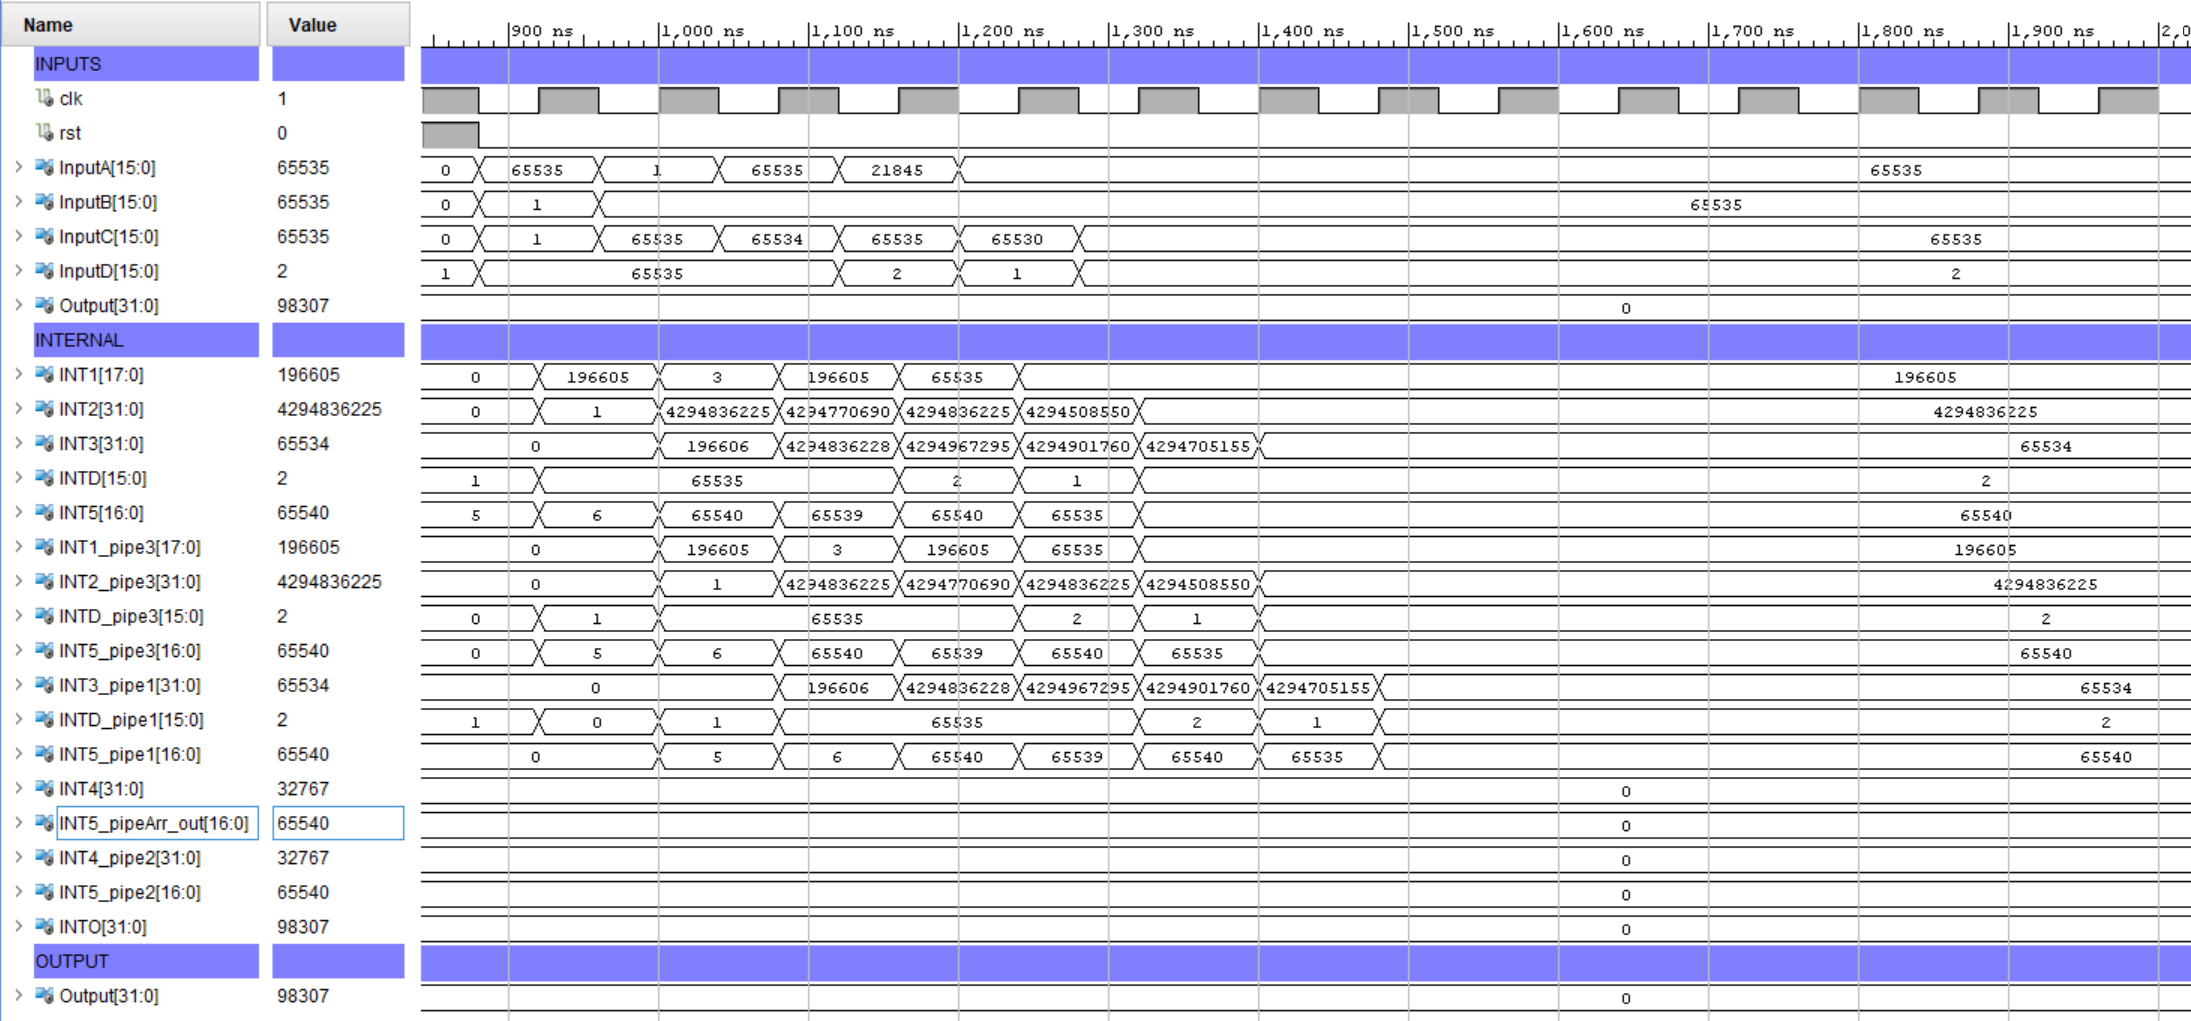
\includegraphics[width=\columnwidth]{Assets/2.2.4_waveform-test-sequence-1.png}
\end{figure}

\subsection*{Waveform 2: Test Sequence 2}
\begin{figure}[H]
    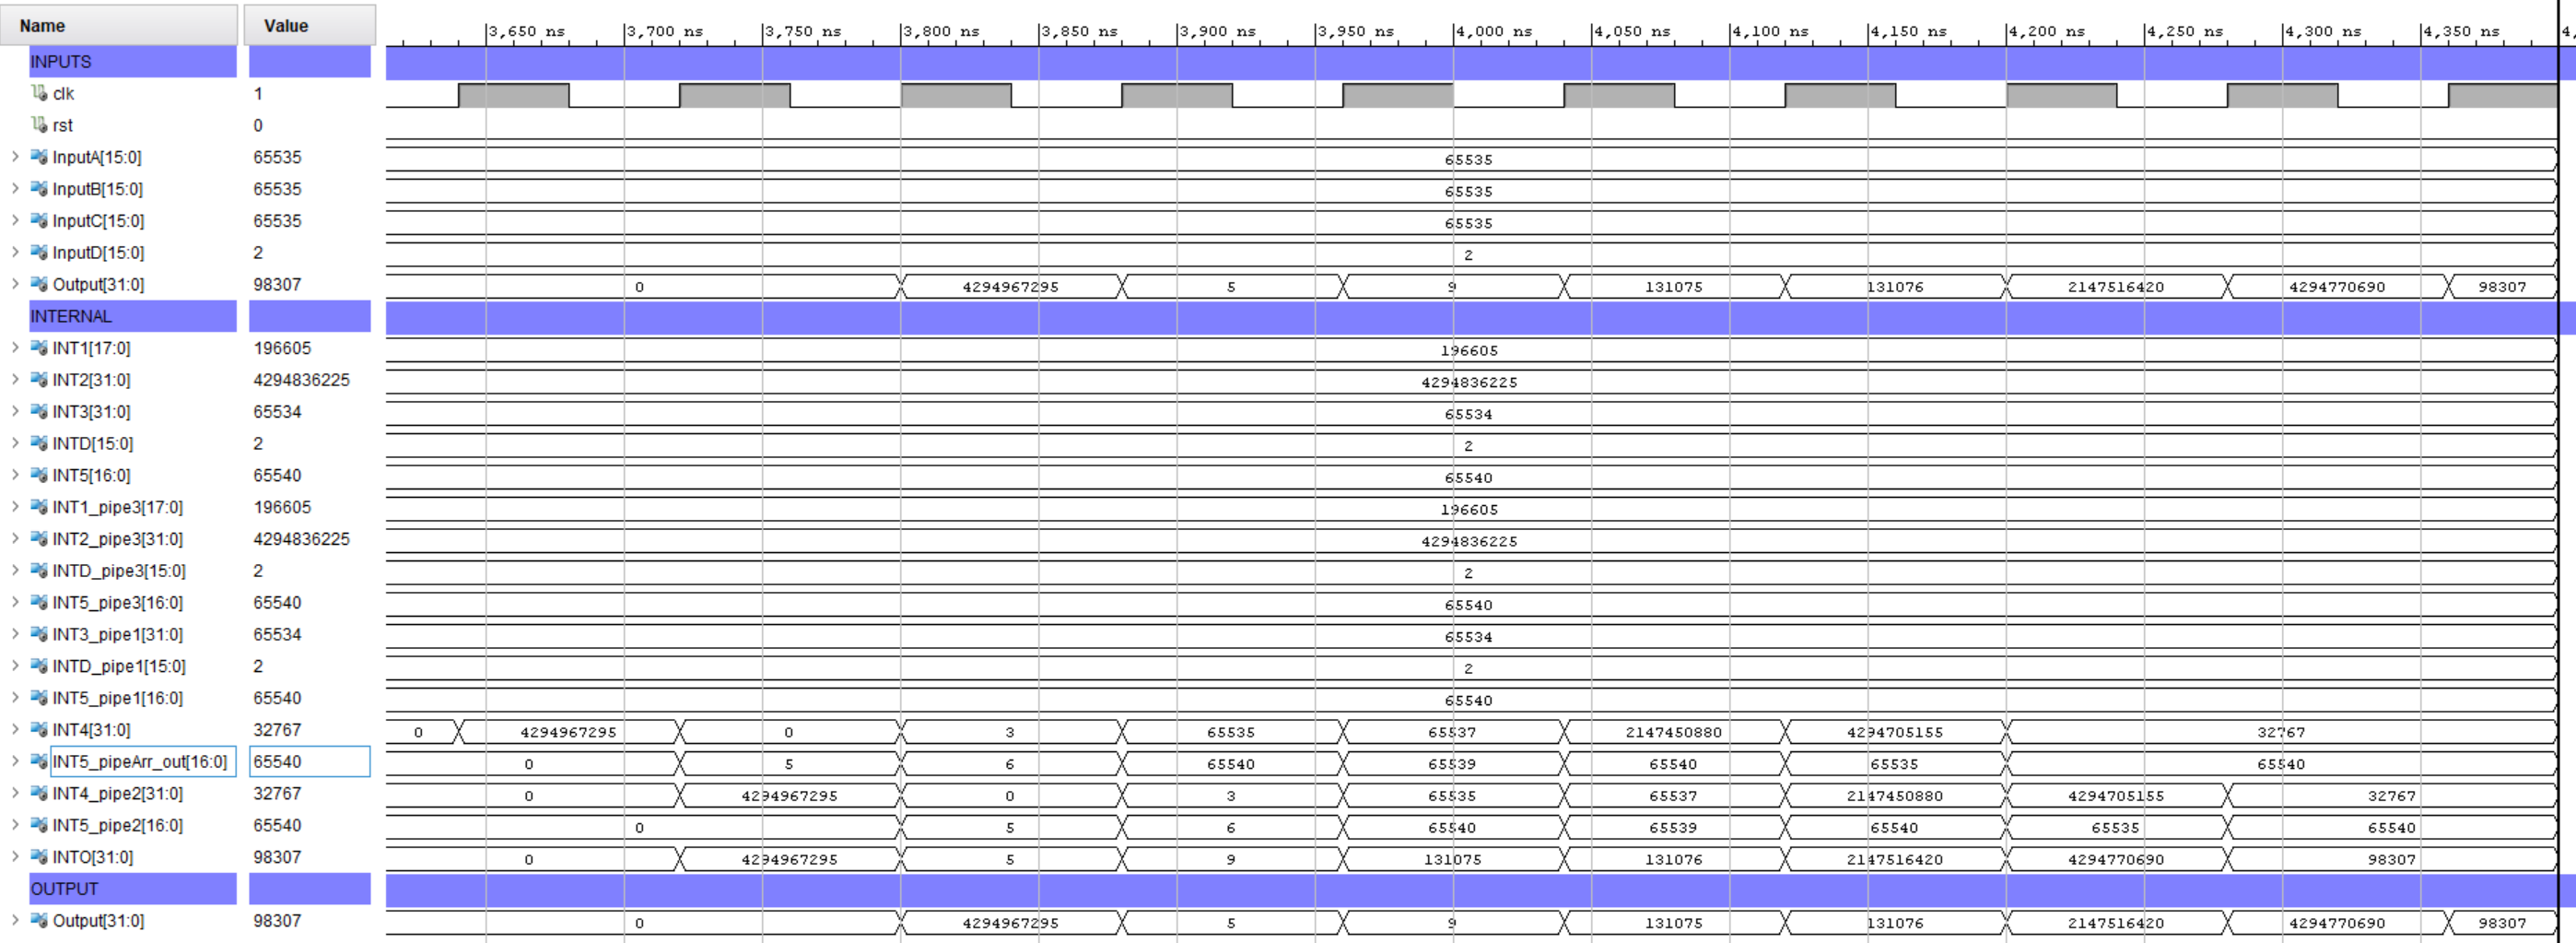
\includegraphics[width=\columnwidth]{Assets/2.2.4_waveform-test-sequence-2.png}
\end{figure}

\subsection*{Console}
\begin{figure}[H]
    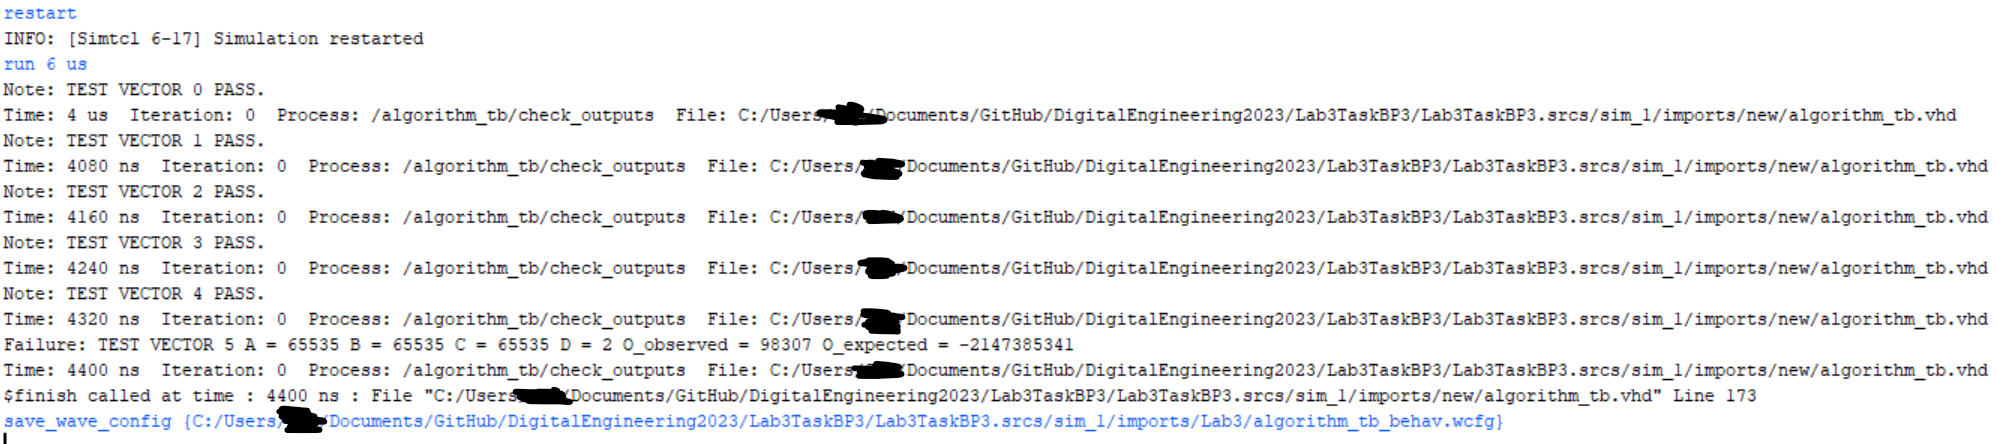
\includegraphics[width=\columnwidth]{Assets/2.2.4_console.png}
\end{figure}

\section*{2.2.5 Design Runs}
\begin{figure}[H]
    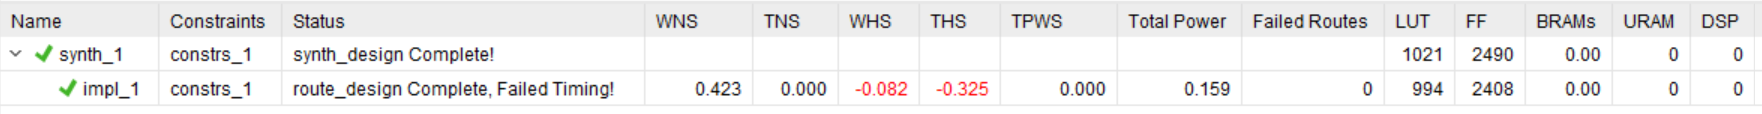
\includegraphics[width=\columnwidth]{Assets/2.2.5_design-runs.png}
\end{figure}
The best period where the constraints are met is at 12ns with a WNS of 0.423ns. The fastest frequency at which this design can run, taking into account the WNS value,
is 86.38MHz

\section*{2.2.6 Post-Route Timing Report: Max Delay Path}
\begin{figure}[H]
    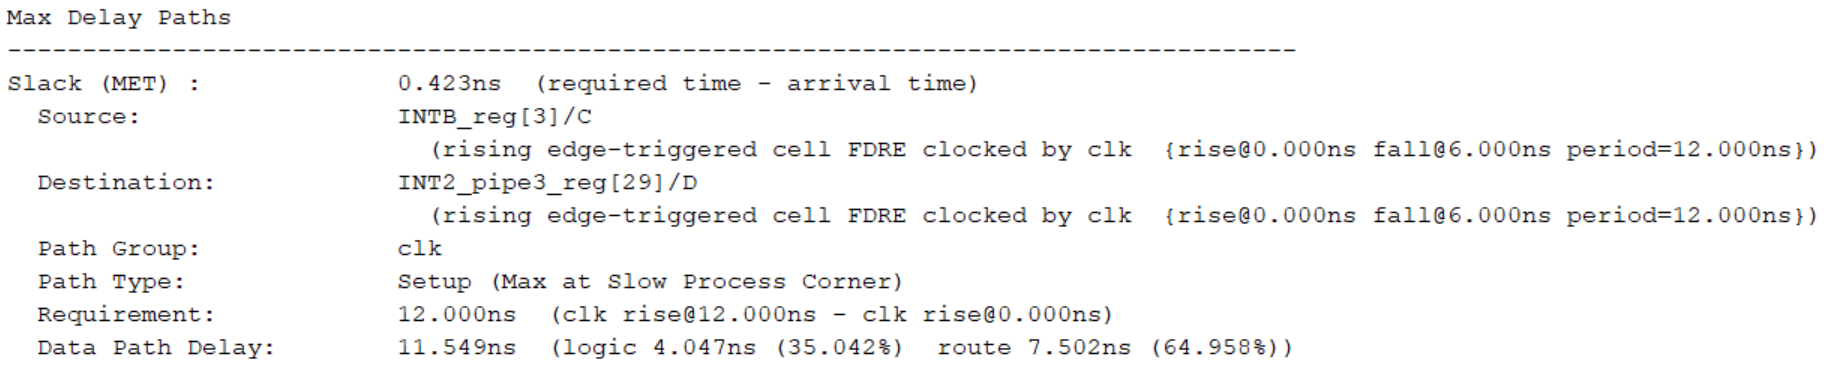
\includegraphics[width=\columnwidth]{Assets/2.2.6_max-delay-path.png}
\end{figure}
From this report, we can identify that the new critical path lies between INTB\_reg and INT2\_pipe3\_reg. This is located in between the input register stage and the third pipeline stage, and the mathematical operation that is within this critical path is the multiplication between inputs B and C.

\section*{2.2.7 Design Runs}
\begin{figure}[H]
    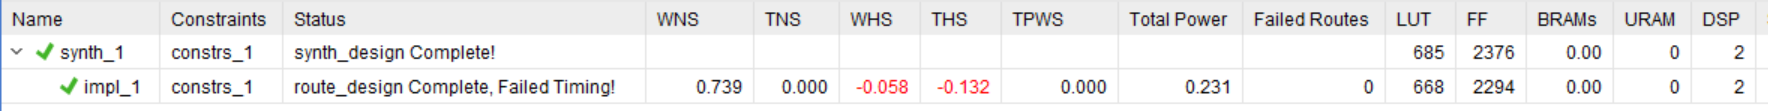
\includegraphics[width=\columnwidth]{Assets/2.2.7_design-runs.png}
\end{figure}
The best period where the constraints are met is at 5ns with a WNS of 0.739ns. The fastest frequency at which this design can run, considering the WNS value, is 234.69MHz.


\section*{2.2.8 Post-Route Timing Report: Max Delay Path}
\begin{figure}[H]
    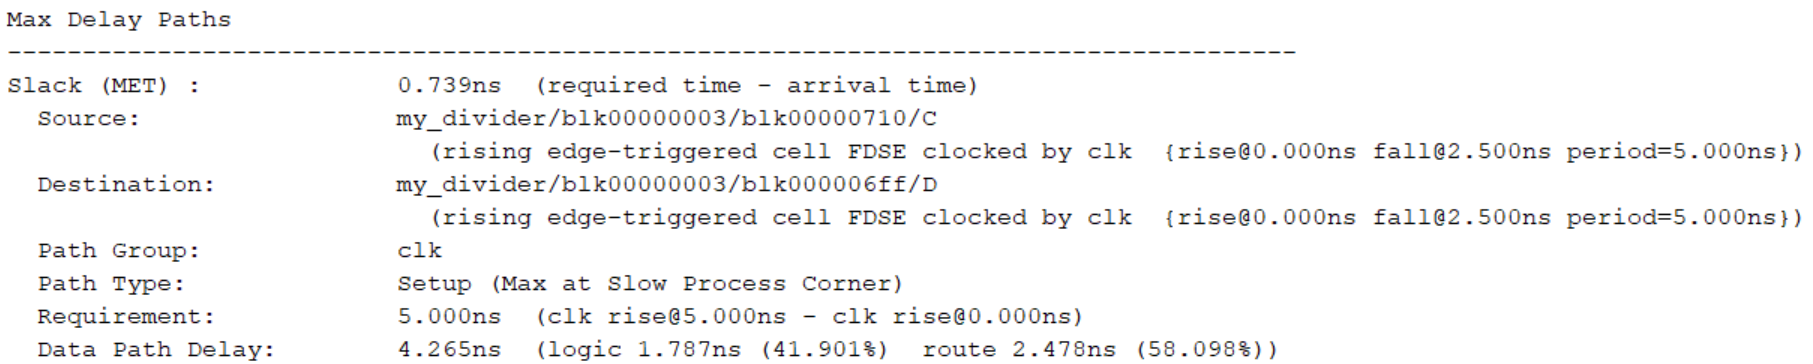
\includegraphics[width=\columnwidth]{Assets/2.2.8_max-delay-path.png}
\end{figure}
From this report, I think I can derive that the new critical path lies within the divider IP block component. This is between the first and second pipeline stages, and parallel to the pipeline array. It isn't much of a surprise to see a divider operation becoming part of the critical path, as the division operation is quite demanding in terms of hardware.

\section*{2.2.9 Code and Component Statistics}
\subsection*{VHDL Code}
\inputminted[firstline=23]{vhdl}{"../../Lab3TaskBP3/Lab3TaskBP3.srcs/sources_1/imports/sources_1/imports/Digital Engineering/Algorithm.vhd"}


\break
\subsection*{RTL Component Statistics}
\inputminted[firstline=94, lastline=101]{text}{"../../Lab3TaskBP3/Lab3TaskBP3.runs/synth_1/algorithm.vds"}

\subsection*{RTL Hierarchical Component Statistics}
\inputminted[firstline=108, lastline=117]{text}{"../../Lab3TaskBP3/Lab3TaskBP3.runs/synth_1/algorithm.vds"}

\end{document}
